\documentclass[twoside]{book}

% Packages required by doxygen
\usepackage{fixltx2e}
\usepackage{calc}
\usepackage{doxygen}
\usepackage[export]{adjustbox} % also loads graphicx
\usepackage{graphicx}
\usepackage[utf8]{inputenc}
\usepackage{makeidx}
\usepackage{multicol}
\usepackage{multirow}
\PassOptionsToPackage{warn}{textcomp}
\usepackage{textcomp}
\usepackage[nointegrals]{wasysym}
\usepackage[table]{xcolor}

% Font selection
\usepackage[T1]{fontenc}
\usepackage[scaled=.90]{helvet}
\usepackage{courier}
\usepackage{amssymb}
\usepackage{sectsty}
\renewcommand{\familydefault}{\sfdefault}
\allsectionsfont{%
  \fontseries{bc}\selectfont%
  \color{darkgray}%
}
\renewcommand{\DoxyLabelFont}{%
  \fontseries{bc}\selectfont%
  \color{darkgray}%
}
\newcommand{\+}{\discretionary{\mbox{\scriptsize$\hookleftarrow$}}{}{}}

% Page & text layout
\usepackage{geometry}
\geometry{%
  a4paper,%
  top=2.5cm,%
  bottom=2.5cm,%
  left=2.5cm,%
  right=2.5cm%
}
\tolerance=750
\hfuzz=15pt
\hbadness=750
\setlength{\emergencystretch}{15pt}
\setlength{\parindent}{0cm}
\setlength{\parskip}{3ex plus 2ex minus 2ex}
\makeatletter
\renewcommand{\paragraph}{%
  \@startsection{paragraph}{4}{0ex}{-1.0ex}{1.0ex}{%
    \normalfont\normalsize\bfseries\SS@parafont%
  }%
}
\renewcommand{\subparagraph}{%
  \@startsection{subparagraph}{5}{0ex}{-1.0ex}{1.0ex}{%
    \normalfont\normalsize\bfseries\SS@subparafont%
  }%
}
\makeatother

% Headers & footers
\usepackage{fancyhdr}
\pagestyle{fancyplain}
\fancyhead[LE]{\fancyplain{}{\bfseries\thepage}}
\fancyhead[CE]{\fancyplain{}{}}
\fancyhead[RE]{\fancyplain{}{\bfseries\leftmark}}
\fancyhead[LO]{\fancyplain{}{\bfseries\rightmark}}
\fancyhead[CO]{\fancyplain{}{}}
\fancyhead[RO]{\fancyplain{}{\bfseries\thepage}}
\fancyfoot[LE]{\fancyplain{}{}}
\fancyfoot[CE]{\fancyplain{}{}}
\fancyfoot[RE]{\fancyplain{}{\bfseries\scriptsize Generated by Doxygen }}
\fancyfoot[LO]{\fancyplain{}{\bfseries\scriptsize Generated by Doxygen }}
\fancyfoot[CO]{\fancyplain{}{}}
\fancyfoot[RO]{\fancyplain{}{}}
\renewcommand{\footrulewidth}{0.4pt}
\renewcommand{\chaptermark}[1]{%
  \markboth{#1}{}%
}
\renewcommand{\sectionmark}[1]{%
  \markright{\thesection\ #1}%
}

% Indices & bibliography
\usepackage{natbib}
\usepackage[titles]{tocloft}
\setcounter{tocdepth}{3}
\setcounter{secnumdepth}{5}
\makeindex

% Hyperlinks (required, but should be loaded last)
\usepackage{ifpdf}
\ifpdf
  \usepackage[pdftex,pagebackref=true]{hyperref}
\else
  \usepackage[ps2pdf,pagebackref=true]{hyperref}
\fi
\hypersetup{%
  colorlinks=true,%
  linkcolor=blue,%
  citecolor=blue,%
  unicode%
}

% Custom commands
\newcommand{\clearemptydoublepage}{%
  \newpage{\pagestyle{empty}\cleardoublepage}%
}

\usepackage{caption}
\captionsetup{labelsep=space,justification=centering,font={bf},singlelinecheck=off,skip=4pt,position=top}

%===== C O N T E N T S =====

\begin{document}

% Titlepage & ToC
\hypersetup{pageanchor=false,
             bookmarksnumbered=true,
             pdfencoding=unicode
            }
\pagenumbering{alph}
\begin{titlepage}
\vspace*{7cm}
\begin{center}%
{\Large Stereo U\+GV \\[1ex]\large 0.\+0.\+0 }\\
\vspace*{1cm}
{\large Generated by Doxygen 1.8.13}\\
\end{center}
\end{titlepage}
\clearemptydoublepage
\pagenumbering{roman}
\tableofcontents
\clearemptydoublepage
\pagenumbering{arabic}
\hypersetup{pageanchor=true}

%--- Begin generated contents ---
\chapter{Namespace Index}
\section{Namespace List}
Here is a list of all documented namespaces with brief descriptions\+:\begin{DoxyCompactList}
\item\contentsline{section}{\hyperlink{namespacestereo__ugv}{stereo\+\_\+ugv} \\*The namespace for public classes and functions of the Stereo U\+GV package }{\pageref{namespacestereo__ugv}}{}
\end{DoxyCompactList}

\chapter{Hierarchical Index}
\section{Class Hierarchy}
This inheritance list is sorted roughly, but not completely, alphabetically\+:\begin{DoxyCompactList}
\item \contentsline{section}{stereo\+\_\+ugv\+:\+:Context}{\pageref{classstereo__ugv_1_1Context}}{}
\item exception\begin{DoxyCompactList}
\item \contentsline{section}{stereo\+\_\+ugv\+:\+:Exception}{\pageref{classstereo__ugv_1_1Exception}}{}
\begin{DoxyCompactList}
\item \contentsline{section}{stereo\+\_\+ugv\+:\+:Invalid\+Parameter}{\pageref{classstereo__ugv_1_1InvalidParameter}}{}
\item \contentsline{section}{stereo\+\_\+ugv\+:\+:Out\+Of\+Frames}{\pageref{classstereo__ugv_1_1OutOfFrames}}{}
\item \contentsline{section}{stereo\+\_\+ugv\+:\+:Parse\+Error}{\pageref{classstereo__ugv_1_1ParseError}}{}
\item \contentsline{section}{stereo\+\_\+ugv\+:\+:Runtime\+Error}{\pageref{classstereo__ugv_1_1RuntimeError}}{}
\end{DoxyCompactList}
\end{DoxyCompactList}
\item \contentsline{section}{stereo\+\_\+ugv\+:\+:Frame\+Layout}{\pageref{classstereo__ugv_1_1FrameLayout}}{}
\begin{DoxyCompactList}
\item \contentsline{section}{stereo\+\_\+ugv\+:\+:H\+P\+S3\+D160\+Frame\+Layout}{\pageref{classstereo__ugv_1_1HPS3D160FrameLayout}}{}
\end{DoxyCompactList}
\item \contentsline{section}{stereo\+\_\+ugv\+:\+:Image\+Source}{\pageref{classstereo__ugv_1_1ImageSource}}{}
\begin{DoxyCompactList}
\item \contentsline{section}{stereo\+\_\+ugv\+:\+:Cv\+Video\+Capture\+Image\+Source$<$ Type $>$}{\pageref{classstereo__ugv_1_1CvVideoCaptureImageSource}}{}
\end{DoxyCompactList}
\item \contentsline{section}{stereo\+\_\+ugv\+:\+:Image\+Undistorter}{\pageref{classstereo__ugv_1_1ImageUndistorter}}{}
\item \contentsline{section}{stereo\+\_\+ugv\+:\+:Lens\+Calibrator}{\pageref{classstereo__ugv_1_1LensCalibrator}}{}
\begin{DoxyCompactList}
\item \contentsline{section}{stereo\+\_\+ugv\+:\+:Chessboard\+Lens\+Calibrator}{\pageref{classstereo__ugv_1_1ChessboardLensCalibrator}}{}
\end{DoxyCompactList}
\item \contentsline{section}{stereo\+\_\+ugv\+:\+:Lens\+Coefficients}{\pageref{structstereo__ugv_1_1LensCoefficients}}{}
\end{DoxyCompactList}

\chapter{Class Index}
\section{Class List}
Here are the classes, structs, unions and interfaces with brief descriptions\+:\begin{DoxyCompactList}
\item\contentsline{section}{\hyperlink{classstereo__ugv_1_1Context}{stereo\+\_\+ugv\+::\+Context} \\*The class for initializing objects from parameters stored in J\+S\+ON files }{\pageref{classstereo__ugv_1_1Context}}{}
\item\contentsline{section}{\hyperlink{classstereo__ugv_1_1Exception}{stereo\+\_\+ugv\+::\+Exception} \\*The base class for exceptions }{\pageref{classstereo__ugv_1_1Exception}}{}
\item\contentsline{section}{\hyperlink{classstereo__ugv_1_1FrameLayout}{stereo\+\_\+ugv\+::\+Frame\+Layout} \\*The base class that defines how images taken by two heads of a stereo camera are positioned in the same frame }{\pageref{classstereo__ugv_1_1FrameLayout}}{}
\item\contentsline{section}{\hyperlink{classstereo__ugv_1_1HPS3D160FrameLayout}{stereo\+\_\+ugv\+::\+H\+P\+S3\+D160\+Frame\+Layout} \\*The class of frame layout for H\+P\+S-\/3\+D160 cameras }{\pageref{classstereo__ugv_1_1HPS3D160FrameLayout}}{}
\item\contentsline{section}{\hyperlink{classstereo__ugv_1_1InvalidParameter}{stereo\+\_\+ugv\+::\+Invalid\+Parameter} \\*The class for errors due to unaccepted initialization parameters }{\pageref{classstereo__ugv_1_1InvalidParameter}}{}
\item\contentsline{section}{\hyperlink{classstereo__ugv_1_1ParseError}{stereo\+\_\+ugv\+::\+Parse\+Error} \\*The class for parse errors encountered during variable substitution on strings within J\+S\+ON }{\pageref{classstereo__ugv_1_1ParseError}}{}
\end{DoxyCompactList}

\chapter{File Index}
\section{File List}
Here is a list of all documented files with brief descriptions\+:\begin{DoxyCompactList}
\item\contentsline{section}{/home/yunhao/stereo\+\_\+ugv/src/stereo\+\_\+ugv/include/stereo\+\_\+ugv/\hyperlink{context_8h}{context.\+h} \\*Defines \hyperlink{classstereo__ugv_1_1Context}{stereo\+\_\+ugv\+::\+Context} and initialization functions of several common types }{\pageref{context_8h}}{}
\item\contentsline{section}{/home/yunhao/stereo\+\_\+ugv/src/stereo\+\_\+ugv/include/stereo\+\_\+ugv/\hyperlink{exception_8h}{exception.\+h} \\*Defines \hyperlink{classstereo__ugv_1_1Exception}{stereo\+\_\+ugv\+::\+Exception} and its subclasses }{\pageref{exception_8h}}{}
\item\contentsline{section}{/home/yunhao/stereo\+\_\+ugv/src/stereo\+\_\+ugv/include/stereo\+\_\+ugv/\hyperlink{frame__layout_8h}{frame\+\_\+layout.\+h} \\*Defines \hyperlink{classstereo__ugv_1_1FrameLayout}{stereo\+\_\+ugv\+::\+Frame\+Layout} and its subclasses }{\pageref{frame__layout_8h}}{}
\item\contentsline{section}{/home/yunhao/stereo\+\_\+ugv/src/stereo\+\_\+ugv/include/stereo\+\_\+ugv/\hyperlink{image__publisher_8h}{image\+\_\+publisher.\+h} \\*Defines stereo\+\_\+ugv\+::\+Image\+Publisher$<$\+T$>$ template class and common image converters }{\pageref{image__publisher_8h}}{}
\item\contentsline{section}{/home/yunhao/stereo\+\_\+ugv/src/stereo\+\_\+ugv/include/stereo\+\_\+ugv/\hyperlink{image__source_8h}{image\+\_\+source.\+h} \\*Defines \hyperlink{classstereo__ugv_1_1ImageSource}{stereo\+\_\+ugv\+::\+Image\+Source} and its subclasses }{\pageref{image__source_8h}}{}
\item\contentsline{section}{/home/yunhao/stereo\+\_\+ugv/src/stereo\+\_\+ugv/include/stereo\+\_\+ugv/\hyperlink{image__undistorter_8h}{image\+\_\+undistorter.\+h} \\*Defines \hyperlink{classstereo__ugv_1_1ImageUndistorter}{stereo\+\_\+ugv\+::\+Image\+Undistorter} }{\pageref{image__undistorter_8h}}{}
\item\contentsline{section}{/home/yunhao/stereo\+\_\+ugv/src/stereo\+\_\+ugv/include/stereo\+\_\+ugv/\hyperlink{lens__calibrator_8h}{lens\+\_\+calibrator.\+h} \\*Defines \hyperlink{classstereo__ugv_1_1LensCalibrator}{stereo\+\_\+ugv\+::\+Lens\+Calibrator} and its subclasses }{\pageref{lens__calibrator_8h}}{}
\end{DoxyCompactList}

\chapter{Namespace Documentation}
\hypertarget{namespacestereo__ugv}{}\section{stereo\+\_\+ugv Namespace Reference}
\label{namespacestereo__ugv}\index{stereo\+\_\+ugv@{stereo\+\_\+ugv}}


The namespace for public classes and functions of the \hyperlink{namespacestereo__ugv}{stereo\+\_\+ugv} package.  


\subsection*{Classes}
\begin{DoxyCompactItemize}
\item 
class \hyperlink{classstereo__ugv_1_1Context}{Context}
\begin{DoxyCompactList}\small\item\em The class for initializing objects from parameters stored in J\+S\+ON files. \end{DoxyCompactList}\item 
class \hyperlink{classstereo__ugv_1_1Exception}{Exception}
\begin{DoxyCompactList}\small\item\em The base class for exceptions. \end{DoxyCompactList}\item 
class \hyperlink{classstereo__ugv_1_1FrameLayout}{Frame\+Layout}
\begin{DoxyCompactList}\small\item\em The base class that defines how images taken by two heads of a stereo camera are positioned in the same frame. \end{DoxyCompactList}\item 
class \hyperlink{classstereo__ugv_1_1HPS3D160FrameLayout}{H\+P\+S3\+D160\+Frame\+Layout}
\begin{DoxyCompactList}\small\item\em The class of frame layout for H\+P\+S-\/3\+D160 cameras. \end{DoxyCompactList}\item 
class \hyperlink{classstereo__ugv_1_1InvalidParameter}{Invalid\+Parameter}
\begin{DoxyCompactList}\small\item\em The class for errors due to unaccepted initialization parameters. \end{DoxyCompactList}\item 
class \hyperlink{classstereo__ugv_1_1OutOfFrames}{Out\+Of\+Frames}
\begin{DoxyCompactList}\small\item\em The class of exception thrown when an image source is running out of frames. \end{DoxyCompactList}\item 
class \hyperlink{classstereo__ugv_1_1ParseError}{Parse\+Error}
\begin{DoxyCompactList}\small\item\em The class for parse errors encountered during variable substitution on strings within J\+S\+ON. \end{DoxyCompactList}\item 
class \hyperlink{classstereo__ugv_1_1RuntimeError}{Runtime\+Error}
\begin{DoxyCompactList}\small\item\em The class for errors that are not due to programming errors and do not have a clear cause. \end{DoxyCompactList}\end{DoxyCompactItemize}
\subsection*{Functions}
\begin{DoxyCompactItemize}
\item 
{\footnotesize template$<$typename T $>$ }\\void \hyperlink{namespacestereo__ugv_a6971cc11001fdf589a71f6fb3099c65b}{initialize} (T $\ast$parameter, const \hyperlink{classstereo__ugv_1_1Context}{Context} \&context)
\begin{DoxyCompactList}\small\item\em Initializes a parameter. \end{DoxyCompactList}\item 
\mbox{\Hypertarget{namespacestereo__ugv_aaa158ec1ee9178414843adbbb91a394b}\label{namespacestereo__ugv_aaa158ec1ee9178414843adbbb91a394b}} 
void {\bfseries initialize} (std\+::string $\ast$string, const \hyperlink{classstereo__ugv_1_1Context}{Context} \&context)
\item 
\mbox{\Hypertarget{namespacestereo__ugv_adab204dc6f43824bcda4cd5e172d2812}\label{namespacestereo__ugv_adab204dc6f43824bcda4cd5e172d2812}} 
void {\bfseries initialize} (cv\+::\+Size $\ast$size, const \hyperlink{classstereo__ugv_1_1Context}{Context} \&context)
\item 
\mbox{\Hypertarget{namespacestereo__ugv_a0a98148c84d1f085ac51c2f2fb7c8e7a}\label{namespacestereo__ugv_a0a98148c84d1f085ac51c2f2fb7c8e7a}} 
void {\bfseries initialize} (cv\+::\+Term\+Criteria $\ast$criteria, const \hyperlink{classstereo__ugv_1_1Context}{Context} \&context)
\item 
\mbox{\Hypertarget{namespacestereo__ugv_aef8f9a951e11f9d5d178db99754aac4b}\label{namespacestereo__ugv_aef8f9a951e11f9d5d178db99754aac4b}} 
\hyperlink{classstereo__ugv_1_1Context}{Context} {\bfseries open\+Internal\+Context} (nlohmann\+::json $\ast$json, const \hyperlink{classstereo__ugv_1_1Context}{Context} \&context)
\item 
\mbox{\Hypertarget{namespacestereo__ugv_ac02cc03581ba53b911a9a7bd87f9a24c}\label{namespacestereo__ugv_ac02cc03581ba53b911a9a7bd87f9a24c}} 
void {\bfseries initialize} (\hyperlink{classstereo__ugv_1_1HPS3D160FrameLayout}{H\+P\+S3\+D160\+Frame\+Layout} $\ast$layout, const \hyperlink{classstereo__ugv_1_1Context}{Context} \&context)
\item 
std\+::string \hyperlink{namespacestereo__ugv_af45c67058883fb26e2c27945af6ab490}{find\+Camera\+Character\+Device\+File} (const std\+::string \&)
\begin{DoxyCompactList}\small\item\em Finds the character device file of a camera device given the prefix of its device name. \end{DoxyCompactList}\end{DoxyCompactItemize}


\subsection{Detailed Description}
The namespace for public classes and functions of the \hyperlink{namespacestereo__ugv}{stereo\+\_\+ugv} package. 

\subsection{Function Documentation}
\mbox{\Hypertarget{namespacestereo__ugv_af45c67058883fb26e2c27945af6ab490}\label{namespacestereo__ugv_af45c67058883fb26e2c27945af6ab490}} 
\index{stereo\+\_\+ugv@{stereo\+\_\+ugv}!find\+Camera\+Character\+Device\+File@{find\+Camera\+Character\+Device\+File}}
\index{find\+Camera\+Character\+Device\+File@{find\+Camera\+Character\+Device\+File}!stereo\+\_\+ugv@{stereo\+\_\+ugv}}
\subsubsection{\texorpdfstring{find\+Camera\+Character\+Device\+File()}{findCameraCharacterDeviceFile()}}
{\footnotesize\ttfamily std\+::string stereo\+\_\+ugv\+::find\+Camera\+Character\+Device\+File (\begin{DoxyParamCaption}\item[{const std\+::string \&}]{ }\end{DoxyParamCaption})}



Finds the character device file of a camera device given the prefix of its device name. 

\begin{DoxyWarning}{Warning}
This function has not been implemented, and calling it will always cause a \hyperlink{classstereo__ugv_1_1RuntimeError}{Runtime\+Error}. 
\end{DoxyWarning}

\begin{DoxyParams}{Parameters}
{\em device\+\_\+name\+\_\+prefix} & The prefix of its device name. Due to the limits of the V4\+L2 A\+PI, device names longer than 31 characters are truncated. Therefore, the length of the given prefix should not be longer than 31 characters. Otherwise, no matching camera can be found. \\
\hline
\end{DoxyParams}
\begin{DoxyReturn}{Returns}
The full path to the character device file. If multiple matching cameras are detected, the function issues a warning and returns any one among them. 
\end{DoxyReturn}
\mbox{\Hypertarget{namespacestereo__ugv_a6971cc11001fdf589a71f6fb3099c65b}\label{namespacestereo__ugv_a6971cc11001fdf589a71f6fb3099c65b}} 
\index{stereo\+\_\+ugv@{stereo\+\_\+ugv}!initialize@{initialize}}
\index{initialize@{initialize}!stereo\+\_\+ugv@{stereo\+\_\+ugv}}
\subsubsection{\texorpdfstring{initialize()}{initialize()}}
{\footnotesize\ttfamily template$<$typename T $>$ \\
void stereo\+\_\+ugv\+::initialize (\begin{DoxyParamCaption}\item[{T $\ast$}]{parameter,  }\item[{const \hyperlink{classstereo__ugv_1_1Context}{Context} \&}]{context }\end{DoxyParamCaption})\hspace{0.3cm}{\ttfamily [inline]}}



Initializes a parameter. 


\begin{DoxyTemplParams}{Template Parameters}
{\em T} & The type of the parameter to be initialized. It should be directly representable by the J\+S\+ON format, e.\+g. boolean, number, string, etc. Otherwise, a custom overload of this function should be defined and used. \\
\hline
\end{DoxyTemplParams}

\begin{DoxyParams}{Parameters}
{\em parameter} & The parameter to be initialized. \\
\hline
{\em context} & The context. \\
\hline
\end{DoxyParams}

\chapter{Class Documentation}
\hypertarget{classstereo__ugv_1_1ChessboardLensCalibrator}{}\section{stereo\+\_\+ugv\+:\+:Chessboard\+Lens\+Calibrator Class Reference}
\label{classstereo__ugv_1_1ChessboardLensCalibrator}\index{stereo\+\_\+ugv\+::\+Chessboard\+Lens\+Calibrator@{stereo\+\_\+ugv\+::\+Chessboard\+Lens\+Calibrator}}


The class for calibrating a stereo camera using a chessboard pattern.  




{\ttfamily \#include $<$lens\+\_\+calibrator.\+h$>$}



Inheritance diagram for stereo\+\_\+ugv\+:\+:Chessboard\+Lens\+Calibrator\+:
\nopagebreak
\begin{figure}[H]
\begin{center}
\leavevmode
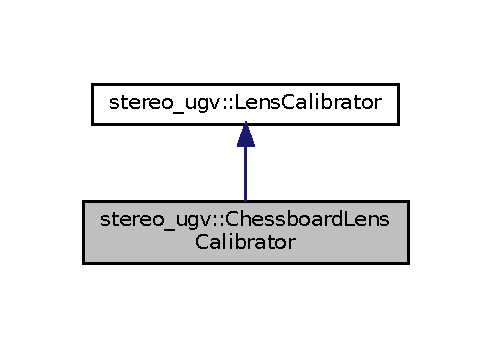
\includegraphics[width=236pt]{classstereo__ugv_1_1ChessboardLensCalibrator__inherit__graph}
\end{center}
\end{figure}


Collaboration diagram for stereo\+\_\+ugv\+:\+:Chessboard\+Lens\+Calibrator\+:
\nopagebreak
\begin{figure}[H]
\begin{center}
\leavevmode
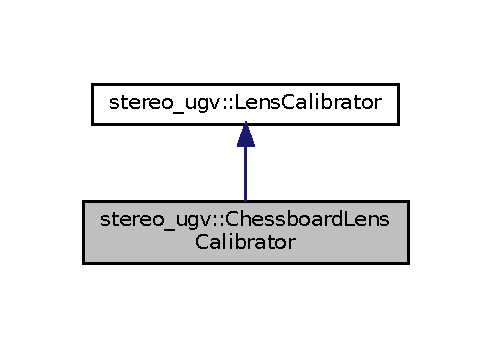
\includegraphics[width=236pt]{classstereo__ugv_1_1ChessboardLensCalibrator__coll__graph}
\end{center}
\end{figure}
\subsection*{Public Member Functions}
\begin{DoxyCompactItemize}
\item 
void \hyperlink{classstereo__ugv_1_1ChessboardLensCalibrator_aeda7a0a6538957e6174277931abf5cd4}{set\+Pattern\+Size} (cv\+::\+Size size)
\begin{DoxyCompactList}\small\item\em Sets the size of the chessboard pattern. \end{DoxyCompactList}\item 
void \hyperlink{classstereo__ugv_1_1ChessboardLensCalibrator_a232059124de2dcb4467bd2a586c75273}{set\+Square\+Length} (float length)
\begin{DoxyCompactList}\small\item\em Sets the square length of the chessboard pattern. \end{DoxyCompactList}\item 
void \hyperlink{classstereo__ugv_1_1ChessboardLensCalibrator_a438ea74bec4002b39dee1985cba88948}{set\+Release\+Object} (bool enabled)
\begin{DoxyCompactList}\small\item\em Sets whether the method of releasing object is enabled. \end{DoxyCompactList}\item 
void \hyperlink{classstereo__ugv_1_1ChessboardLensCalibrator_af2814fa1b58cdb9b2a8c3a1c46113da8}{set\+Marker} (bool enabled)
\begin{DoxyCompactList}\small\item\em Sets whether the chessboard pattern has markers. \end{DoxyCompactList}\end{DoxyCompactItemize}
\subsection*{Protected Member Functions}
\begin{DoxyCompactItemize}
\item 
virtual bool \hyperlink{classstereo__ugv_1_1ChessboardLensCalibrator_ac6e93519a72d4218bcb1f9a49a9c22eb}{detect\+Image\+Points} (const cv\+::\+Mat \&image, std\+::vector$<$ cv\+::\+Point2f $>$ $\ast$points) const override
\begin{DoxyCompactList}\small\item\em Detects feature points in the given image. \end{DoxyCompactList}\item 
virtual std\+::vector$<$ cv\+::\+Point3f $>$ \hyperlink{classstereo__ugv_1_1ChessboardLensCalibrator_adaeaa9e0a3203872ea8e5ef5b3482f7e}{create\+Object\+Points} () const override
\begin{DoxyCompactList}\small\item\em Creates the 3D points corresponding to the detected 2D points in images. \end{DoxyCompactList}\item 
virtual int \hyperlink{classstereo__ugv_1_1ChessboardLensCalibrator_a00aa88f3399b59ec686f6d506c73a910}{index\+Of\+Fixed\+Point} () const noexcept override
\begin{DoxyCompactList}\small\item\em Gets the index of the fixed point if the method of releasing object is used. \end{DoxyCompactList}\end{DoxyCompactItemize}
\subsection*{Additional Inherited Members}


\subsection{Detailed Description}
The class for calibrating a stereo camera using a chessboard pattern. 

\subsection{Member Function Documentation}
\mbox{\Hypertarget{classstereo__ugv_1_1ChessboardLensCalibrator_adaeaa9e0a3203872ea8e5ef5b3482f7e}\label{classstereo__ugv_1_1ChessboardLensCalibrator_adaeaa9e0a3203872ea8e5ef5b3482f7e}} 
\index{stereo\+\_\+ugv\+::\+Chessboard\+Lens\+Calibrator@{stereo\+\_\+ugv\+::\+Chessboard\+Lens\+Calibrator}!create\+Object\+Points@{create\+Object\+Points}}
\index{create\+Object\+Points@{create\+Object\+Points}!stereo\+\_\+ugv\+::\+Chessboard\+Lens\+Calibrator@{stereo\+\_\+ugv\+::\+Chessboard\+Lens\+Calibrator}}
\subsubsection{\texorpdfstring{create\+Object\+Points()}{createObjectPoints()}}
{\footnotesize\ttfamily std\+::vector$<$ cv\+::\+Point3f $>$ stereo\+\_\+ugv\+::\+Chessboard\+Lens\+Calibrator\+::create\+Object\+Points (\begin{DoxyParamCaption}{ }\end{DoxyParamCaption}) const\hspace{0.3cm}{\ttfamily [override]}, {\ttfamily [protected]}, {\ttfamily [virtual]}}



Creates the 3D points corresponding to the detected 2D points in images. 

\begin{DoxyReturn}{Returns}
A vector of 3D points. 
\end{DoxyReturn}


Implements \hyperlink{classstereo__ugv_1_1LensCalibrator_a3edf81dfc9567904a0d1a7c3555d65bf}{stereo\+\_\+ugv\+::\+Lens\+Calibrator}.

\mbox{\Hypertarget{classstereo__ugv_1_1ChessboardLensCalibrator_ac6e93519a72d4218bcb1f9a49a9c22eb}\label{classstereo__ugv_1_1ChessboardLensCalibrator_ac6e93519a72d4218bcb1f9a49a9c22eb}} 
\index{stereo\+\_\+ugv\+::\+Chessboard\+Lens\+Calibrator@{stereo\+\_\+ugv\+::\+Chessboard\+Lens\+Calibrator}!detect\+Image\+Points@{detect\+Image\+Points}}
\index{detect\+Image\+Points@{detect\+Image\+Points}!stereo\+\_\+ugv\+::\+Chessboard\+Lens\+Calibrator@{stereo\+\_\+ugv\+::\+Chessboard\+Lens\+Calibrator}}
\subsubsection{\texorpdfstring{detect\+Image\+Points()}{detectImagePoints()}}
{\footnotesize\ttfamily bool stereo\+\_\+ugv\+::\+Chessboard\+Lens\+Calibrator\+::detect\+Image\+Points (\begin{DoxyParamCaption}\item[{const cv\+::\+Mat \&}]{image,  }\item[{std\+::vector$<$ cv\+::\+Point2f $>$ $\ast$}]{points }\end{DoxyParamCaption}) const\hspace{0.3cm}{\ttfamily [override]}, {\ttfamily [protected]}, {\ttfamily [virtual]}}



Detects feature points in the given image. 

The number of detected points must be constant, and these 2D points should corresponds to fixed points on a roughly planar rigid body in 3D space. 
\begin{DoxyParams}{Parameters}
{\em image} & The image. \\
\hline
{\em points} & The feature points to be detected. It will not be assigned if no feature points were detected. \\
\hline
\end{DoxyParams}
\begin{DoxyReturn}{Returns}
Whether feature points are detected. 
\end{DoxyReturn}


Implements \hyperlink{classstereo__ugv_1_1LensCalibrator_a9be834b0ef2983af47ac5f9dd67887fe}{stereo\+\_\+ugv\+::\+Lens\+Calibrator}.

\mbox{\Hypertarget{classstereo__ugv_1_1ChessboardLensCalibrator_a00aa88f3399b59ec686f6d506c73a910}\label{classstereo__ugv_1_1ChessboardLensCalibrator_a00aa88f3399b59ec686f6d506c73a910}} 
\index{stereo\+\_\+ugv\+::\+Chessboard\+Lens\+Calibrator@{stereo\+\_\+ugv\+::\+Chessboard\+Lens\+Calibrator}!index\+Of\+Fixed\+Point@{index\+Of\+Fixed\+Point}}
\index{index\+Of\+Fixed\+Point@{index\+Of\+Fixed\+Point}!stereo\+\_\+ugv\+::\+Chessboard\+Lens\+Calibrator@{stereo\+\_\+ugv\+::\+Chessboard\+Lens\+Calibrator}}
\subsubsection{\texorpdfstring{index\+Of\+Fixed\+Point()}{indexOfFixedPoint()}}
{\footnotesize\ttfamily int stereo\+\_\+ugv\+::\+Chessboard\+Lens\+Calibrator\+::index\+Of\+Fixed\+Point (\begin{DoxyParamCaption}{ }\end{DoxyParamCaption}) const\hspace{0.3cm}{\ttfamily [override]}, {\ttfamily [protected]}, {\ttfamily [virtual]}, {\ttfamily [noexcept]}}



Gets the index of the fixed point if the method of releasing object is used. 

\begin{DoxyReturn}{Returns}
If the traditional calibration method is used, returns 0. Otherwise if the method of releasing object is used, return the index of the fixed point which is between 1 and number\+\_\+of\+\_\+points -\/ 1. 
\end{DoxyReturn}


Implements \hyperlink{classstereo__ugv_1_1LensCalibrator_ad25267d7b60a912f270701359eda1c54}{stereo\+\_\+ugv\+::\+Lens\+Calibrator}.

\mbox{\Hypertarget{classstereo__ugv_1_1ChessboardLensCalibrator_af2814fa1b58cdb9b2a8c3a1c46113da8}\label{classstereo__ugv_1_1ChessboardLensCalibrator_af2814fa1b58cdb9b2a8c3a1c46113da8}} 
\index{stereo\+\_\+ugv\+::\+Chessboard\+Lens\+Calibrator@{stereo\+\_\+ugv\+::\+Chessboard\+Lens\+Calibrator}!set\+Marker@{set\+Marker}}
\index{set\+Marker@{set\+Marker}!stereo\+\_\+ugv\+::\+Chessboard\+Lens\+Calibrator@{stereo\+\_\+ugv\+::\+Chessboard\+Lens\+Calibrator}}
\subsubsection{\texorpdfstring{set\+Marker()}{setMarker()}}
{\footnotesize\ttfamily void stereo\+\_\+ugv\+::\+Chessboard\+Lens\+Calibrator\+::set\+Marker (\begin{DoxyParamCaption}\item[{bool}]{enabled }\end{DoxyParamCaption})}



Sets whether the chessboard pattern has markers. 


\begin{DoxyParams}{Parameters}
{\em enabled} & Whether the chessboard pattern has markers. \\
\hline
\end{DoxyParams}
\mbox{\Hypertarget{classstereo__ugv_1_1ChessboardLensCalibrator_aeda7a0a6538957e6174277931abf5cd4}\label{classstereo__ugv_1_1ChessboardLensCalibrator_aeda7a0a6538957e6174277931abf5cd4}} 
\index{stereo\+\_\+ugv\+::\+Chessboard\+Lens\+Calibrator@{stereo\+\_\+ugv\+::\+Chessboard\+Lens\+Calibrator}!set\+Pattern\+Size@{set\+Pattern\+Size}}
\index{set\+Pattern\+Size@{set\+Pattern\+Size}!stereo\+\_\+ugv\+::\+Chessboard\+Lens\+Calibrator@{stereo\+\_\+ugv\+::\+Chessboard\+Lens\+Calibrator}}
\subsubsection{\texorpdfstring{set\+Pattern\+Size()}{setPatternSize()}}
{\footnotesize\ttfamily void stereo\+\_\+ugv\+::\+Chessboard\+Lens\+Calibrator\+::set\+Pattern\+Size (\begin{DoxyParamCaption}\item[{cv\+::\+Size}]{size }\end{DoxyParamCaption})}



Sets the size of the chessboard pattern. 


\begin{DoxyParams}{Parameters}
{\em size} & The pattern size. \\
\hline
\end{DoxyParams}
\mbox{\Hypertarget{classstereo__ugv_1_1ChessboardLensCalibrator_a438ea74bec4002b39dee1985cba88948}\label{classstereo__ugv_1_1ChessboardLensCalibrator_a438ea74bec4002b39dee1985cba88948}} 
\index{stereo\+\_\+ugv\+::\+Chessboard\+Lens\+Calibrator@{stereo\+\_\+ugv\+::\+Chessboard\+Lens\+Calibrator}!set\+Release\+Object@{set\+Release\+Object}}
\index{set\+Release\+Object@{set\+Release\+Object}!stereo\+\_\+ugv\+::\+Chessboard\+Lens\+Calibrator@{stereo\+\_\+ugv\+::\+Chessboard\+Lens\+Calibrator}}
\subsubsection{\texorpdfstring{set\+Release\+Object()}{setReleaseObject()}}
{\footnotesize\ttfamily void stereo\+\_\+ugv\+::\+Chessboard\+Lens\+Calibrator\+::set\+Release\+Object (\begin{DoxyParamCaption}\item[{bool}]{enabled }\end{DoxyParamCaption})}



Sets whether the method of releasing object is enabled. 

If the method of releasing object is enabled, the last point of the first row will be chosen as the third fixed point in cv\+::calibrate\+Camera\+R\+O(). 
\begin{DoxyParams}{Parameters}
{\em enabled} & Whether the method of releasing object is enabled. \\
\hline
\end{DoxyParams}
\mbox{\Hypertarget{classstereo__ugv_1_1ChessboardLensCalibrator_a232059124de2dcb4467bd2a586c75273}\label{classstereo__ugv_1_1ChessboardLensCalibrator_a232059124de2dcb4467bd2a586c75273}} 
\index{stereo\+\_\+ugv\+::\+Chessboard\+Lens\+Calibrator@{stereo\+\_\+ugv\+::\+Chessboard\+Lens\+Calibrator}!set\+Square\+Length@{set\+Square\+Length}}
\index{set\+Square\+Length@{set\+Square\+Length}!stereo\+\_\+ugv\+::\+Chessboard\+Lens\+Calibrator@{stereo\+\_\+ugv\+::\+Chessboard\+Lens\+Calibrator}}
\subsubsection{\texorpdfstring{set\+Square\+Length()}{setSquareLength()}}
{\footnotesize\ttfamily void stereo\+\_\+ugv\+::\+Chessboard\+Lens\+Calibrator\+::set\+Square\+Length (\begin{DoxyParamCaption}\item[{float}]{length }\end{DoxyParamCaption})}



Sets the square length of the chessboard pattern. 


\begin{DoxyParams}{Parameters}
{\em length} & The square length. \\
\hline
\end{DoxyParams}


The documentation for this class was generated from the following files\+:\begin{DoxyCompactItemize}
\item 
/home/yunhao/stereo\+\_\+ugv/src/stereo\+\_\+ugv/include/stereo\+\_\+ugv/\hyperlink{lens__calibrator_8h}{lens\+\_\+calibrator.\+h}\item 
/home/yunhao/stereo\+\_\+ugv/src/stereo\+\_\+ugv/src/stereo\+\_\+ugv/lens\+\_\+calibrator.\+cpp\end{DoxyCompactItemize}

\hypertarget{classstereo__ugv_1_1Context}{}\section{stereo\+\_\+ugv\+:\+:Context Class Reference}
\label{classstereo__ugv_1_1Context}\index{stereo\+\_\+ugv\+::\+Context@{stereo\+\_\+ugv\+::\+Context}}


The class for initializing objects from parameters stored in J\+S\+ON files.  




{\ttfamily \#include $<$context.\+h$>$}

\subsection*{Public Member Functions}
\begin{DoxyCompactItemize}
\item 
\hyperlink{classstereo__ugv_1_1Context_a408832fdf3245f3d91c9ea794ebbc71c}{Context} (const nlohmann\+::json $\ast$parameter\+\_\+json, const std\+::unordered\+\_\+map$<$ std\+::string, std\+::string $>$ $\ast$variable\+\_\+map, image\+\_\+transport\+::\+Image\+Transport $\ast$image\+\_\+transport) noexcept
\begin{DoxyCompactList}\small\item\em Creates a context. \end{DoxyCompactList}\item 
\hyperlink{classstereo__ugv_1_1Context_a2c89fdaa8a60d2b8d1dae87e11142f03}{Context} (const \hyperlink{classstereo__ugv_1_1Context}{Context} \&other, const std\+::string \&key)
\begin{DoxyCompactList}\small\item\em Creates a new context based on the given original context, except that the new underlying J\+S\+ON is the child of the original underlying J\+S\+ON at the given key. \end{DoxyCompactList}\item 
const nlohmann\+::json \& \hyperlink{classstereo__ugv_1_1Context_a6b40977abc9924a49282b26e05d866aa}{parameter\+J\+S\+ON} () const noexcept
\begin{DoxyCompactList}\small\item\em Gets the J\+S\+ON object that stores parameters for object initialization. \end{DoxyCompactList}\item 
const std\+::unordered\+\_\+map$<$ std\+::string, std\+::string $>$ \& \hyperlink{classstereo__ugv_1_1Context_a0071b4b8bc7f1b9a5c1ce541a68334e0}{variable\+Map} () const noexcept
\begin{DoxyCompactList}\small\item\em Gets the map for performing variable substitution on strings. \end{DoxyCompactList}\item 
image\+\_\+transport\+::\+Image\+Transport \& \hyperlink{classstereo__ugv_1_1Context_a62b2e85a2c109ff079324fe5fbf0fe92}{image\+Transport} () const noexcept
\begin{DoxyCompactList}\small\item\em Gets the image transport for creating image publishers. \end{DoxyCompactList}\item 
{\footnotesize template$<$typename T $>$ }\\void \hyperlink{classstereo__ugv_1_1Context_a1996f3d3213ab26a3ba84a1c0cf7b62e}{get\+Parameter} (const std\+::string \&key, T $\ast$parameter) const
\begin{DoxyCompactList}\small\item\em Initializes the parameter of the given key. \end{DoxyCompactList}\item 
{\footnotesize template$<$typename T $>$ }\\void \hyperlink{classstereo__ugv_1_1Context_a8e7e25d1efa5c92a84830824c0effa27}{get\+Parameter} (const std\+::string \&key, T $\ast$parameter, const T \&default\+\_\+value) const
\begin{DoxyCompactList}\small\item\em Initializes the parameter of the given key, or assigns it with the default value if the key does not exist. \end{DoxyCompactList}\end{DoxyCompactItemize}


\subsection{Detailed Description}
The class for initializing objects from parameters stored in J\+S\+ON files. 

\subsection{Constructor \& Destructor Documentation}
\mbox{\Hypertarget{classstereo__ugv_1_1Context_a408832fdf3245f3d91c9ea794ebbc71c}\label{classstereo__ugv_1_1Context_a408832fdf3245f3d91c9ea794ebbc71c}} 
\index{stereo\+\_\+ugv\+::\+Context@{stereo\+\_\+ugv\+::\+Context}!Context@{Context}}
\index{Context@{Context}!stereo\+\_\+ugv\+::\+Context@{stereo\+\_\+ugv\+::\+Context}}
\subsubsection{\texorpdfstring{Context()}{Context()}\hspace{0.1cm}{\footnotesize\ttfamily [1/2]}}
{\footnotesize\ttfamily stereo\+\_\+ugv\+::\+Context\+::\+Context (\begin{DoxyParamCaption}\item[{const nlohmann\+::json $\ast$}]{parameter\+\_\+json,  }\item[{const std\+::unordered\+\_\+map$<$ std\+::string, std\+::string $>$ $\ast$}]{variable\+\_\+map,  }\item[{image\+\_\+transport\+::\+Image\+Transport $\ast$}]{image\+\_\+transport }\end{DoxyParamCaption})\hspace{0.3cm}{\ttfamily [noexcept]}}



Creates a context. 


\begin{DoxyParams}{Parameters}
{\em parameter\+\_\+json} & A J\+S\+ON object that stores parameters for object initialization. \\
\hline
{\em variable\+\_\+map} & A key-\/value map for performing variable substitution on strings within J\+S\+ON. \\
\hline
{\em image\+\_\+transport} & An image transport for creating image publishers. \\
\hline
\end{DoxyParams}
\mbox{\Hypertarget{classstereo__ugv_1_1Context_a2c89fdaa8a60d2b8d1dae87e11142f03}\label{classstereo__ugv_1_1Context_a2c89fdaa8a60d2b8d1dae87e11142f03}} 
\index{stereo\+\_\+ugv\+::\+Context@{stereo\+\_\+ugv\+::\+Context}!Context@{Context}}
\index{Context@{Context}!stereo\+\_\+ugv\+::\+Context@{stereo\+\_\+ugv\+::\+Context}}
\subsubsection{\texorpdfstring{Context()}{Context()}\hspace{0.1cm}{\footnotesize\ttfamily [2/2]}}
{\footnotesize\ttfamily stereo\+\_\+ugv\+::\+Context\+::\+Context (\begin{DoxyParamCaption}\item[{const \hyperlink{classstereo__ugv_1_1Context}{Context} \&}]{other,  }\item[{const std\+::string \&}]{key }\end{DoxyParamCaption})}



Creates a new context based on the given original context, except that the new underlying J\+S\+ON is the child of the original underlying J\+S\+ON at the given key. 


\begin{DoxyParams}{Parameters}
{\em other} & The original context. \\
\hline
{\em key} & The key of the original underlying J\+S\+ON object. \\
\hline
\end{DoxyParams}


\subsection{Member Function Documentation}
\mbox{\Hypertarget{classstereo__ugv_1_1Context_a1996f3d3213ab26a3ba84a1c0cf7b62e}\label{classstereo__ugv_1_1Context_a1996f3d3213ab26a3ba84a1c0cf7b62e}} 
\index{stereo\+\_\+ugv\+::\+Context@{stereo\+\_\+ugv\+::\+Context}!get\+Parameter@{get\+Parameter}}
\index{get\+Parameter@{get\+Parameter}!stereo\+\_\+ugv\+::\+Context@{stereo\+\_\+ugv\+::\+Context}}
\subsubsection{\texorpdfstring{get\+Parameter()}{getParameter()}\hspace{0.1cm}{\footnotesize\ttfamily [1/2]}}
{\footnotesize\ttfamily template$<$typename T $>$ \\
void stereo\+\_\+ugv\+::\+Context\+::get\+Parameter (\begin{DoxyParamCaption}\item[{const std\+::string \&}]{key,  }\item[{T $\ast$}]{parameter }\end{DoxyParamCaption}) const\hspace{0.3cm}{\ttfamily [inline]}}



Initializes the parameter of the given key. 


\begin{DoxyTemplParams}{Template Parameters}
{\em T} & The type of the parameter to be initialized. The \hyperlink{namespacestereo__ugv_a6971cc11001fdf589a71f6fb3099c65b}{initialize(\+T$\ast$, const Context\&)} function is required. The initialization function should be defined in the same namespace as type T so that it can be found using argument-\/dependent lookup (A\+DL). \\
\hline
\end{DoxyTemplParams}

\begin{DoxyParams}{Parameters}
{\em key} & The key at which the initialization parameters are stored. \\
\hline
{\em parameter} & The parameter to be initialized. \\
\hline
\end{DoxyParams}
\mbox{\Hypertarget{classstereo__ugv_1_1Context_a8e7e25d1efa5c92a84830824c0effa27}\label{classstereo__ugv_1_1Context_a8e7e25d1efa5c92a84830824c0effa27}} 
\index{stereo\+\_\+ugv\+::\+Context@{stereo\+\_\+ugv\+::\+Context}!get\+Parameter@{get\+Parameter}}
\index{get\+Parameter@{get\+Parameter}!stereo\+\_\+ugv\+::\+Context@{stereo\+\_\+ugv\+::\+Context}}
\subsubsection{\texorpdfstring{get\+Parameter()}{getParameter()}\hspace{0.1cm}{\footnotesize\ttfamily [2/2]}}
{\footnotesize\ttfamily template$<$typename T $>$ \\
void stereo\+\_\+ugv\+::\+Context\+::get\+Parameter (\begin{DoxyParamCaption}\item[{const std\+::string \&}]{key,  }\item[{T $\ast$}]{parameter,  }\item[{const T \&}]{default\+\_\+value }\end{DoxyParamCaption}) const\hspace{0.3cm}{\ttfamily [inline]}}



Initializes the parameter of the given key, or assigns it with the default value if the key does not exist. 


\begin{DoxyTemplParams}{Template Parameters}
{\em T} & The type of the parameter to be initialized. The \hyperlink{namespacestereo__ugv_a6971cc11001fdf589a71f6fb3099c65b}{initialize(\+T$\ast$, const Context\&)} function is required. The initialization function should be defined in the same namespace as type T so that it can be found using argument-\/dependent lookup (A\+DL). \\
\hline
\end{DoxyTemplParams}

\begin{DoxyParams}{Parameters}
{\em key} & The key at which the initialization parameters are stored. \\
\hline
{\em parameter} & The parameter to be initialized. \\
\hline
{\em default\+\_\+value} & The default value used when the given key does not exist. \\
\hline
\end{DoxyParams}
\mbox{\Hypertarget{classstereo__ugv_1_1Context_a62b2e85a2c109ff079324fe5fbf0fe92}\label{classstereo__ugv_1_1Context_a62b2e85a2c109ff079324fe5fbf0fe92}} 
\index{stereo\+\_\+ugv\+::\+Context@{stereo\+\_\+ugv\+::\+Context}!image\+Transport@{image\+Transport}}
\index{image\+Transport@{image\+Transport}!stereo\+\_\+ugv\+::\+Context@{stereo\+\_\+ugv\+::\+Context}}
\subsubsection{\texorpdfstring{image\+Transport()}{imageTransport()}}
{\footnotesize\ttfamily image\+\_\+transport\+::\+Image\+Transport \& stereo\+\_\+ugv\+::\+Context\+::image\+Transport (\begin{DoxyParamCaption}{ }\end{DoxyParamCaption}) const\hspace{0.3cm}{\ttfamily [noexcept]}}



Gets the image transport for creating image publishers. 

\begin{DoxyReturn}{Returns}
The image transport. 
\end{DoxyReturn}
\mbox{\Hypertarget{classstereo__ugv_1_1Context_a6b40977abc9924a49282b26e05d866aa}\label{classstereo__ugv_1_1Context_a6b40977abc9924a49282b26e05d866aa}} 
\index{stereo\+\_\+ugv\+::\+Context@{stereo\+\_\+ugv\+::\+Context}!parameter\+J\+S\+ON@{parameter\+J\+S\+ON}}
\index{parameter\+J\+S\+ON@{parameter\+J\+S\+ON}!stereo\+\_\+ugv\+::\+Context@{stereo\+\_\+ugv\+::\+Context}}
\subsubsection{\texorpdfstring{parameter\+J\+S\+O\+N()}{parameterJSON()}}
{\footnotesize\ttfamily const nlohmann\+::json \& stereo\+\_\+ugv\+::\+Context\+::parameter\+J\+S\+ON (\begin{DoxyParamCaption}{ }\end{DoxyParamCaption}) const\hspace{0.3cm}{\ttfamily [noexcept]}}



Gets the J\+S\+ON object that stores parameters for object initialization. 

\begin{DoxyReturn}{Returns}
The J\+S\+ON object. 
\end{DoxyReturn}
\mbox{\Hypertarget{classstereo__ugv_1_1Context_a0071b4b8bc7f1b9a5c1ce541a68334e0}\label{classstereo__ugv_1_1Context_a0071b4b8bc7f1b9a5c1ce541a68334e0}} 
\index{stereo\+\_\+ugv\+::\+Context@{stereo\+\_\+ugv\+::\+Context}!variable\+Map@{variable\+Map}}
\index{variable\+Map@{variable\+Map}!stereo\+\_\+ugv\+::\+Context@{stereo\+\_\+ugv\+::\+Context}}
\subsubsection{\texorpdfstring{variable\+Map()}{variableMap()}}
{\footnotesize\ttfamily const std\+::unordered\+\_\+map$<$ std\+::string, std\+::string $>$ \& stereo\+\_\+ugv\+::\+Context\+::variable\+Map (\begin{DoxyParamCaption}{ }\end{DoxyParamCaption}) const\hspace{0.3cm}{\ttfamily [noexcept]}}



Gets the map for performing variable substitution on strings. 

\begin{DoxyReturn}{Returns}
The map. 
\end{DoxyReturn}


The documentation for this class was generated from the following files\+:\begin{DoxyCompactItemize}
\item 
/home/yunhao/stereo\+\_\+ugv/src/stereo\+\_\+ugv/include/stereo\+\_\+ugv/\hyperlink{context_8h}{context.\+h}\item 
/home/yunhao/stereo\+\_\+ugv/src/stereo\+\_\+ugv/src/stereo\+\_\+ugv/context.\+cpp\end{DoxyCompactItemize}

\hypertarget{classstereo__ugv_1_1CvVideoCaptureImageSource}{}\section{stereo\+\_\+ugv\+:\+:Cv\+Video\+Capture\+Image\+Source$<$ Type $>$ Class Template Reference}
\label{classstereo__ugv_1_1CvVideoCaptureImageSource}\index{stereo\+\_\+ugv\+::\+Cv\+Video\+Capture\+Image\+Source$<$ Type $>$@{stereo\+\_\+ugv\+::\+Cv\+Video\+Capture\+Image\+Source$<$ Type $>$}}


Class for image sources backended by cv\+::\+Video\+Capture.  




{\ttfamily \#include $<$image\+\_\+source.\+h$>$}



Inheritance diagram for stereo\+\_\+ugv\+:\+:Cv\+Video\+Capture\+Image\+Source$<$ Type $>$\+:
\nopagebreak
\begin{figure}[H]
\begin{center}
\leavevmode
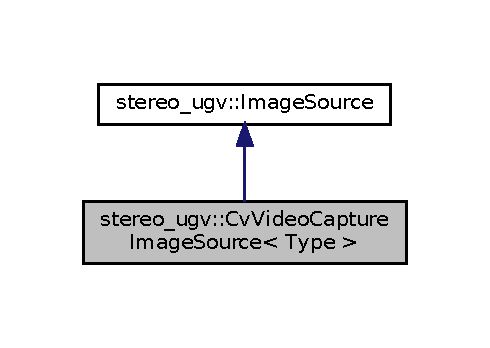
\includegraphics[width=235pt]{classstereo__ugv_1_1CvVideoCaptureImageSource__inherit__graph}
\end{center}
\end{figure}


Collaboration diagram for stereo\+\_\+ugv\+:\+:Cv\+Video\+Capture\+Image\+Source$<$ Type $>$\+:
\nopagebreak
\begin{figure}[H]
\begin{center}
\leavevmode
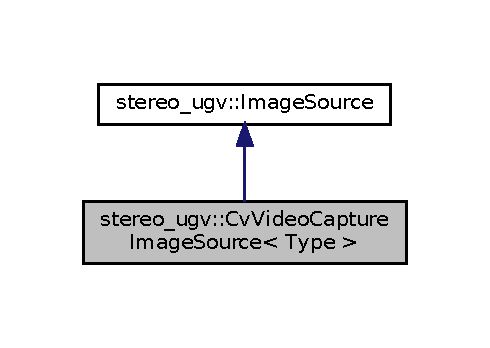
\includegraphics[width=235pt]{classstereo__ugv_1_1CvVideoCaptureImageSource__coll__graph}
\end{center}
\end{figure}
\subsection*{Public Member Functions}
\begin{DoxyCompactItemize}
\item 
void \hyperlink{classstereo__ugv_1_1CvVideoCaptureImageSource_a70f8c34dd228771d141fee7027cbc211}{set\+Frame\+Layout} (std\+::unique\+\_\+ptr$<$ \hyperlink{classstereo__ugv_1_1FrameLayout}{Frame\+Layout} $>$ \&\&layout)
\begin{DoxyCompactList}\small\item\em Sets the frame layout. \end{DoxyCompactList}\item 
void \hyperlink{classstereo__ugv_1_1CvVideoCaptureImageSource_a47e4a18163b03d4d716284292dbb1d24}{open\+Video\+Capture} (const std\+::string \&filename)
\begin{DoxyCompactList}\small\item\em Opens the video capture at the given filename. \end{DoxyCompactList}\item 
virtual cv\+::\+Size \hyperlink{classstereo__ugv_1_1CvVideoCaptureImageSource_a84dd7dbd0ff6091d68843ca02a18e0cc}{image\+Size} () const override
\begin{DoxyCompactList}\small\item\em Gets the image size. The Stereo U\+GV package assumes that images taken by two heads of a stereo camera have the same size. \end{DoxyCompactList}\item 
virtual void \hyperlink{classstereo__ugv_1_1CvVideoCaptureImageSource_a6636c97811bb28d59453c3865b0bda69}{read\+Images} (cv\+::\+Mat $\ast$left, cv\+::\+Mat $\ast$right) override
\begin{DoxyCompactList}\small\item\em Reads a pair of images of the next frame. The Stereo U\+GV package assumes that two heads of a stereo camera are aligned horizontally. \end{DoxyCompactList}\end{DoxyCompactItemize}
\subsection*{Additional Inherited Members}


\subsection{Detailed Description}
\subsubsection*{template$<$Cv\+Video\+Capture\+Type Type$>$\newline
class stereo\+\_\+ugv\+::\+Cv\+Video\+Capture\+Image\+Source$<$ Type $>$}

Class for image sources backended by cv\+::\+Video\+Capture. 


\begin{DoxyTemplParams}{Template Parameters}
{\em Type} & The type of image source. \\
\hline
\end{DoxyTemplParams}


\subsection{Member Function Documentation}
\mbox{\Hypertarget{classstereo__ugv_1_1CvVideoCaptureImageSource_a84dd7dbd0ff6091d68843ca02a18e0cc}\label{classstereo__ugv_1_1CvVideoCaptureImageSource_a84dd7dbd0ff6091d68843ca02a18e0cc}} 
\index{stereo\+\_\+ugv\+::\+Cv\+Video\+Capture\+Image\+Source@{stereo\+\_\+ugv\+::\+Cv\+Video\+Capture\+Image\+Source}!image\+Size@{image\+Size}}
\index{image\+Size@{image\+Size}!stereo\+\_\+ugv\+::\+Cv\+Video\+Capture\+Image\+Source@{stereo\+\_\+ugv\+::\+Cv\+Video\+Capture\+Image\+Source}}
\subsubsection{\texorpdfstring{image\+Size()}{imageSize()}}
{\footnotesize\ttfamily template$<$Cv\+Video\+Capture\+Type Type$>$ \\
virtual cv\+::\+Size \hyperlink{classstereo__ugv_1_1CvVideoCaptureImageSource}{stereo\+\_\+ugv\+::\+Cv\+Video\+Capture\+Image\+Source}$<$ Type $>$\+::image\+Size (\begin{DoxyParamCaption}{ }\end{DoxyParamCaption}) const\hspace{0.3cm}{\ttfamily [inline]}, {\ttfamily [override]}, {\ttfamily [virtual]}}



Gets the image size. The Stereo U\+GV package assumes that images taken by two heads of a stereo camera have the same size. 

\begin{DoxyReturn}{Returns}
The image size. 
\end{DoxyReturn}


Implements \hyperlink{classstereo__ugv_1_1ImageSource_a30d9146abcdcef11f03685a9887b96d0}{stereo\+\_\+ugv\+::\+Image\+Source}.

\mbox{\Hypertarget{classstereo__ugv_1_1CvVideoCaptureImageSource_a47e4a18163b03d4d716284292dbb1d24}\label{classstereo__ugv_1_1CvVideoCaptureImageSource_a47e4a18163b03d4d716284292dbb1d24}} 
\index{stereo\+\_\+ugv\+::\+Cv\+Video\+Capture\+Image\+Source@{stereo\+\_\+ugv\+::\+Cv\+Video\+Capture\+Image\+Source}!open\+Video\+Capture@{open\+Video\+Capture}}
\index{open\+Video\+Capture@{open\+Video\+Capture}!stereo\+\_\+ugv\+::\+Cv\+Video\+Capture\+Image\+Source@{stereo\+\_\+ugv\+::\+Cv\+Video\+Capture\+Image\+Source}}
\subsubsection{\texorpdfstring{open\+Video\+Capture()}{openVideoCapture()}}
{\footnotesize\ttfamily template$<$Cv\+Video\+Capture\+Type Type$>$ \\
void \hyperlink{classstereo__ugv_1_1CvVideoCaptureImageSource}{stereo\+\_\+ugv\+::\+Cv\+Video\+Capture\+Image\+Source}$<$ Type $>$\+::open\+Video\+Capture (\begin{DoxyParamCaption}\item[{const std\+::string \&}]{filename }\end{DoxyParamCaption})\hspace{0.3cm}{\ttfamily [inline]}}



Opens the video capture at the given filename. 

\begin{DoxyWarning}{Warning}
The frame layout must be set before calling this method, because this method relies on the frame layout to provide the frame size used to initialize the image source. 
\end{DoxyWarning}

\begin{DoxyParams}{Parameters}
{\em filename} & If the type is C\+A\+M\+E\+RA, it is the name of the character device file. If the type if I\+M\+A\+G\+ES, it is the pattern of the image sequence filenames. If the type if V\+I\+D\+EO, it is the name of the video file. \\
\hline
\end{DoxyParams}
\mbox{\Hypertarget{classstereo__ugv_1_1CvVideoCaptureImageSource_a6636c97811bb28d59453c3865b0bda69}\label{classstereo__ugv_1_1CvVideoCaptureImageSource_a6636c97811bb28d59453c3865b0bda69}} 
\index{stereo\+\_\+ugv\+::\+Cv\+Video\+Capture\+Image\+Source@{stereo\+\_\+ugv\+::\+Cv\+Video\+Capture\+Image\+Source}!read\+Images@{read\+Images}}
\index{read\+Images@{read\+Images}!stereo\+\_\+ugv\+::\+Cv\+Video\+Capture\+Image\+Source@{stereo\+\_\+ugv\+::\+Cv\+Video\+Capture\+Image\+Source}}
\subsubsection{\texorpdfstring{read\+Images()}{readImages()}}
{\footnotesize\ttfamily template$<$Cv\+Video\+Capture\+Type Type$>$ \\
virtual void \hyperlink{classstereo__ugv_1_1CvVideoCaptureImageSource}{stereo\+\_\+ugv\+::\+Cv\+Video\+Capture\+Image\+Source}$<$ Type $>$\+::read\+Images (\begin{DoxyParamCaption}\item[{cv\+::\+Mat $\ast$}]{left,  }\item[{cv\+::\+Mat $\ast$}]{right }\end{DoxyParamCaption})\hspace{0.3cm}{\ttfamily [inline]}, {\ttfamily [override]}, {\ttfamily [virtual]}}



Reads a pair of images of the next frame. The Stereo U\+GV package assumes that two heads of a stereo camera are aligned horizontally. 


\begin{DoxyParams}{Parameters}
{\em left} & The image taken by the left head. \\
\hline
{\em right} & The image taken by the right head. \\
\hline
\end{DoxyParams}


Implements \hyperlink{classstereo__ugv_1_1ImageSource_a3d87f7b09cd8889fcbee3efb29a0c39c}{stereo\+\_\+ugv\+::\+Image\+Source}.

\mbox{\Hypertarget{classstereo__ugv_1_1CvVideoCaptureImageSource_a70f8c34dd228771d141fee7027cbc211}\label{classstereo__ugv_1_1CvVideoCaptureImageSource_a70f8c34dd228771d141fee7027cbc211}} 
\index{stereo\+\_\+ugv\+::\+Cv\+Video\+Capture\+Image\+Source@{stereo\+\_\+ugv\+::\+Cv\+Video\+Capture\+Image\+Source}!set\+Frame\+Layout@{set\+Frame\+Layout}}
\index{set\+Frame\+Layout@{set\+Frame\+Layout}!stereo\+\_\+ugv\+::\+Cv\+Video\+Capture\+Image\+Source@{stereo\+\_\+ugv\+::\+Cv\+Video\+Capture\+Image\+Source}}
\subsubsection{\texorpdfstring{set\+Frame\+Layout()}{setFrameLayout()}}
{\footnotesize\ttfamily template$<$Cv\+Video\+Capture\+Type Type$>$ \\
void \hyperlink{classstereo__ugv_1_1CvVideoCaptureImageSource}{stereo\+\_\+ugv\+::\+Cv\+Video\+Capture\+Image\+Source}$<$ Type $>$\+::set\+Frame\+Layout (\begin{DoxyParamCaption}\item[{std\+::unique\+\_\+ptr$<$ \hyperlink{classstereo__ugv_1_1FrameLayout}{Frame\+Layout} $>$ \&\&}]{layout }\end{DoxyParamCaption})\hspace{0.3cm}{\ttfamily [inline]}}



Sets the frame layout. 


\begin{DoxyParams}{Parameters}
{\em layout} & The frame layout. \\
\hline
\end{DoxyParams}


The documentation for this class was generated from the following file\+:\begin{DoxyCompactItemize}
\item 
/home/yunhao/stereo\+\_\+ugv/src/stereo\+\_\+ugv/include/stereo\+\_\+ugv/\hyperlink{image__source_8h}{image\+\_\+source.\+h}\end{DoxyCompactItemize}

\hypertarget{classstereo__ugv_1_1Exception}{}\section{stereo\+\_\+ugv\+:\+:Exception Class Reference}
\label{classstereo__ugv_1_1Exception}\index{stereo\+\_\+ugv\+::\+Exception@{stereo\+\_\+ugv\+::\+Exception}}


The base class for exceptions.  




{\ttfamily \#include $<$exception.\+h$>$}



Inheritance diagram for stereo\+\_\+ugv\+:\+:Exception\+:
\nopagebreak
\begin{figure}[H]
\begin{center}
\leavevmode
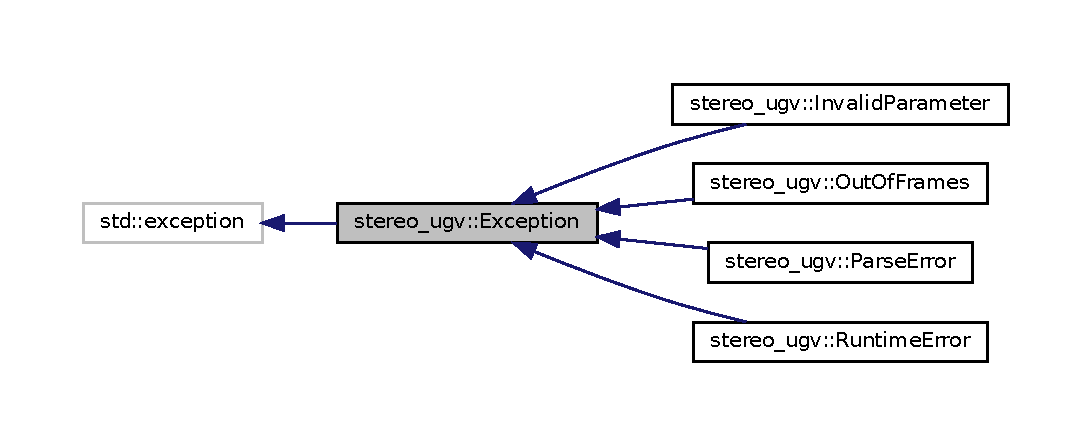
\includegraphics[width=350pt]{classstereo__ugv_1_1Exception__inherit__graph}
\end{center}
\end{figure}


Collaboration diagram for stereo\+\_\+ugv\+:\+:Exception\+:
\nopagebreak
\begin{figure}[H]
\begin{center}
\leavevmode
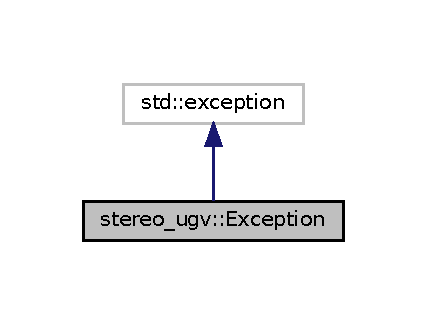
\includegraphics[width=205pt]{classstereo__ugv_1_1Exception__coll__graph}
\end{center}
\end{figure}
\subsection*{Public Member Functions}
\begin{DoxyCompactItemize}
\item 
\hyperlink{classstereo__ugv_1_1Exception_a70f09c97d92872832efce71bd37aabce}{Exception} (const char $\ast$message)
\begin{DoxyCompactList}\small\item\em Creates an exception. \end{DoxyCompactList}\item 
\hyperlink{classstereo__ugv_1_1Exception_a8d813f3fb347af4b3682c2a4bc22d59b}{Exception} (const std\+::string \&message)
\begin{DoxyCompactList}\small\item\em Creates an exception. \end{DoxyCompactList}\item 
virtual const char $\ast$ \hyperlink{classstereo__ugv_1_1Exception_a6222ba0a0cd622e7b560f8dcadf2ec87}{what} () const noexcept override
\begin{DoxyCompactList}\small\item\em Gets the explanatory string. \end{DoxyCompactList}\end{DoxyCompactItemize}


\subsection{Detailed Description}
The base class for exceptions. 

\subsection{Constructor \& Destructor Documentation}
\mbox{\Hypertarget{classstereo__ugv_1_1Exception_a70f09c97d92872832efce71bd37aabce}\label{classstereo__ugv_1_1Exception_a70f09c97d92872832efce71bd37aabce}} 
\index{stereo\+\_\+ugv\+::\+Exception@{stereo\+\_\+ugv\+::\+Exception}!Exception@{Exception}}
\index{Exception@{Exception}!stereo\+\_\+ugv\+::\+Exception@{stereo\+\_\+ugv\+::\+Exception}}
\subsubsection{\texorpdfstring{Exception()}{Exception()}\hspace{0.1cm}{\footnotesize\ttfamily [1/2]}}
{\footnotesize\ttfamily stereo\+\_\+ugv\+::\+Exception\+::\+Exception (\begin{DoxyParamCaption}\item[{const char $\ast$}]{message }\end{DoxyParamCaption})}



Creates an exception. 


\begin{DoxyParams}{Parameters}
{\em message} & The explanatory string. It should be U\+T\+F-\/8 encoded and null-\/terminated. \\
\hline
\end{DoxyParams}
\mbox{\Hypertarget{classstereo__ugv_1_1Exception_a8d813f3fb347af4b3682c2a4bc22d59b}\label{classstereo__ugv_1_1Exception_a8d813f3fb347af4b3682c2a4bc22d59b}} 
\index{stereo\+\_\+ugv\+::\+Exception@{stereo\+\_\+ugv\+::\+Exception}!Exception@{Exception}}
\index{Exception@{Exception}!stereo\+\_\+ugv\+::\+Exception@{stereo\+\_\+ugv\+::\+Exception}}
\subsubsection{\texorpdfstring{Exception()}{Exception()}\hspace{0.1cm}{\footnotesize\ttfamily [2/2]}}
{\footnotesize\ttfamily stereo\+\_\+ugv\+::\+Exception\+::\+Exception (\begin{DoxyParamCaption}\item[{const std\+::string \&}]{message }\end{DoxyParamCaption})}



Creates an exception. 


\begin{DoxyParams}{Parameters}
{\em message} & The U\+T\+F-\/8 encoded explanatory string. \\
\hline
\end{DoxyParams}


\subsection{Member Function Documentation}
\mbox{\Hypertarget{classstereo__ugv_1_1Exception_a6222ba0a0cd622e7b560f8dcadf2ec87}\label{classstereo__ugv_1_1Exception_a6222ba0a0cd622e7b560f8dcadf2ec87}} 
\index{stereo\+\_\+ugv\+::\+Exception@{stereo\+\_\+ugv\+::\+Exception}!what@{what}}
\index{what@{what}!stereo\+\_\+ugv\+::\+Exception@{stereo\+\_\+ugv\+::\+Exception}}
\subsubsection{\texorpdfstring{what()}{what()}}
{\footnotesize\ttfamily const char $\ast$ stereo\+\_\+ugv\+::\+Exception\+::what (\begin{DoxyParamCaption}{ }\end{DoxyParamCaption}) const\hspace{0.3cm}{\ttfamily [override]}, {\ttfamily [virtual]}, {\ttfamily [noexcept]}}



Gets the explanatory string. 

\begin{DoxyReturn}{Returns}
The explanatory string. 
\end{DoxyReturn}


The documentation for this class was generated from the following files\+:\begin{DoxyCompactItemize}
\item 
/home/yunhao/stereo\+\_\+ugv/src/stereo\+\_\+ugv/include/stereo\+\_\+ugv/\hyperlink{exception_8h}{exception.\+h}\item 
/home/yunhao/stereo\+\_\+ugv/src/stereo\+\_\+ugv/src/stereo\+\_\+ugv/exception.\+cpp\end{DoxyCompactItemize}

\hypertarget{classstereo__ugv_1_1FrameLayout}{}\section{stereo\+\_\+ugv\+:\+:Frame\+Layout Class Reference}
\label{classstereo__ugv_1_1FrameLayout}\index{stereo\+\_\+ugv\+::\+Frame\+Layout@{stereo\+\_\+ugv\+::\+Frame\+Layout}}


The base class that defines how images taken by two heads of a stereo camera are positioned in the same frame.  




{\ttfamily \#include $<$frame\+\_\+layout.\+h$>$}



Inheritance diagram for stereo\+\_\+ugv\+:\+:Frame\+Layout\+:\nopagebreak
\begin{figure}[H]
\begin{center}
\leavevmode
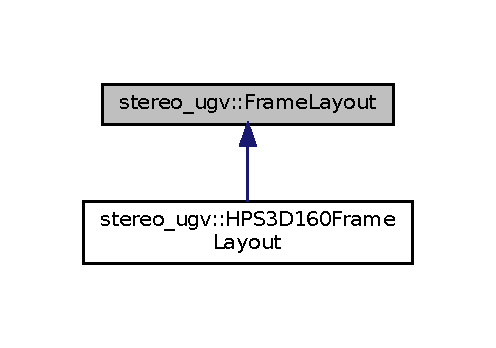
\includegraphics[width=238pt]{classstereo__ugv_1_1FrameLayout__inherit__graph}
\end{center}
\end{figure}
\subsection*{Public Member Functions}
\begin{DoxyCompactItemize}
\item 
virtual cv\+::\+Size \hyperlink{classstereo__ugv_1_1FrameLayout_a59da4ac9d0cc6a43cccbf8666849bdc2}{frame\+Size} () const =0
\begin{DoxyCompactList}\small\item\em Gets the frame size. \end{DoxyCompactList}\item 
virtual cv\+::\+Size \hyperlink{classstereo__ugv_1_1FrameLayout_a12cc36a89f8e66ffc6a2fa5eb3c5f648}{image\+Size} () const =0
\begin{DoxyCompactList}\small\item\em Gets the image size. The Stereo U\+GV package assumes that images taken by two heads of a stereo camera have the same size. \end{DoxyCompactList}\item 
virtual void \hyperlink{classstereo__ugv_1_1FrameLayout_af5ab49a35cfbb59a79863720e7985d29}{extract\+Images} (const cv\+::\+Mat \&frame, cv\+::\+Mat $\ast$left, cv\+::\+Mat $\ast$right) const =0
\begin{DoxyCompactList}\small\item\em Extracts images from the given frame. The Stereo U\+GV package assumes that two heads of a stereo camera are aligned horizontally. \end{DoxyCompactList}\end{DoxyCompactItemize}
\subsection*{Static Public Member Functions}
\begin{DoxyCompactItemize}
\item 
static std\+::unique\+\_\+ptr$<$ \hyperlink{classstereo__ugv_1_1FrameLayout}{Frame\+Layout} $>$ \hyperlink{classstereo__ugv_1_1FrameLayout_adaaac30572f6e3b6fc88da66873c2e77}{create} (const \hyperlink{classstereo__ugv_1_1Context}{Context} \&context)
\begin{DoxyCompactList}\small\item\em Creates a \hyperlink{classstereo__ugv_1_1FrameLayout}{Frame\+Layout}. \end{DoxyCompactList}\end{DoxyCompactItemize}


\subsection{Detailed Description}
The base class that defines how images taken by two heads of a stereo camera are positioned in the same frame. 

\subsection{Member Function Documentation}
\mbox{\Hypertarget{classstereo__ugv_1_1FrameLayout_adaaac30572f6e3b6fc88da66873c2e77}\label{classstereo__ugv_1_1FrameLayout_adaaac30572f6e3b6fc88da66873c2e77}} 
\index{stereo\+\_\+ugv\+::\+Frame\+Layout@{stereo\+\_\+ugv\+::\+Frame\+Layout}!create@{create}}
\index{create@{create}!stereo\+\_\+ugv\+::\+Frame\+Layout@{stereo\+\_\+ugv\+::\+Frame\+Layout}}
\subsubsection{\texorpdfstring{create()}{create()}}
{\footnotesize\ttfamily std\+::unique\+\_\+ptr$<$ \hyperlink{classstereo__ugv_1_1FrameLayout}{Frame\+Layout} $>$ stereo\+\_\+ugv\+::\+Frame\+Layout\+::create (\begin{DoxyParamCaption}\item[{const \hyperlink{classstereo__ugv_1_1Context}{Context} \&}]{context }\end{DoxyParamCaption})\hspace{0.3cm}{\ttfamily [static]}}



Creates a \hyperlink{classstereo__ugv_1_1FrameLayout}{Frame\+Layout}. 

The function determines the concrete subclass of the layout to be created by looking up the \char`\"{}type\char`\"{} key, and calls the corresponding initialization function. Currently, only \char`\"{}\+H\+P\+S-\/3\+D160\char`\"{} is supported. 
\begin{DoxyParams}{Parameters}
{\em context} & The context containing initialization parameters. \\
\hline
\end{DoxyParams}
\begin{DoxyReturn}{Returns}
A unique pointer to the created layout. 
\end{DoxyReturn}
\mbox{\Hypertarget{classstereo__ugv_1_1FrameLayout_af5ab49a35cfbb59a79863720e7985d29}\label{classstereo__ugv_1_1FrameLayout_af5ab49a35cfbb59a79863720e7985d29}} 
\index{stereo\+\_\+ugv\+::\+Frame\+Layout@{stereo\+\_\+ugv\+::\+Frame\+Layout}!extract\+Images@{extract\+Images}}
\index{extract\+Images@{extract\+Images}!stereo\+\_\+ugv\+::\+Frame\+Layout@{stereo\+\_\+ugv\+::\+Frame\+Layout}}
\subsubsection{\texorpdfstring{extract\+Images()}{extractImages()}}
{\footnotesize\ttfamily virtual void stereo\+\_\+ugv\+::\+Frame\+Layout\+::extract\+Images (\begin{DoxyParamCaption}\item[{const cv\+::\+Mat \&}]{frame,  }\item[{cv\+::\+Mat $\ast$}]{left,  }\item[{cv\+::\+Mat $\ast$}]{right }\end{DoxyParamCaption}) const\hspace{0.3cm}{\ttfamily [pure virtual]}}



Extracts images from the given frame. The Stereo U\+GV package assumes that two heads of a stereo camera are aligned horizontally. 


\begin{DoxyParams}{Parameters}
{\em frame} & The frame. \\
\hline
{\em left} & The left image to be extracted. \\
\hline
{\em right} & The right image to be extracted. \\
\hline
\end{DoxyParams}


Implemented in \hyperlink{classstereo__ugv_1_1HPS3D160FrameLayout_a224d3fddea38c0c564baa8d391a396fa}{stereo\+\_\+ugv\+::\+H\+P\+S3\+D160\+Frame\+Layout}.

\mbox{\Hypertarget{classstereo__ugv_1_1FrameLayout_a59da4ac9d0cc6a43cccbf8666849bdc2}\label{classstereo__ugv_1_1FrameLayout_a59da4ac9d0cc6a43cccbf8666849bdc2}} 
\index{stereo\+\_\+ugv\+::\+Frame\+Layout@{stereo\+\_\+ugv\+::\+Frame\+Layout}!frame\+Size@{frame\+Size}}
\index{frame\+Size@{frame\+Size}!stereo\+\_\+ugv\+::\+Frame\+Layout@{stereo\+\_\+ugv\+::\+Frame\+Layout}}
\subsubsection{\texorpdfstring{frame\+Size()}{frameSize()}}
{\footnotesize\ttfamily virtual cv\+::\+Size stereo\+\_\+ugv\+::\+Frame\+Layout\+::frame\+Size (\begin{DoxyParamCaption}{ }\end{DoxyParamCaption}) const\hspace{0.3cm}{\ttfamily [pure virtual]}}



Gets the frame size. 

\begin{DoxyReturn}{Returns}
The frame size. 
\end{DoxyReturn}


Implemented in \hyperlink{classstereo__ugv_1_1HPS3D160FrameLayout_add697132a4d32b0f1fc49f35f3b8fa0f}{stereo\+\_\+ugv\+::\+H\+P\+S3\+D160\+Frame\+Layout}.

\mbox{\Hypertarget{classstereo__ugv_1_1FrameLayout_a12cc36a89f8e66ffc6a2fa5eb3c5f648}\label{classstereo__ugv_1_1FrameLayout_a12cc36a89f8e66ffc6a2fa5eb3c5f648}} 
\index{stereo\+\_\+ugv\+::\+Frame\+Layout@{stereo\+\_\+ugv\+::\+Frame\+Layout}!image\+Size@{image\+Size}}
\index{image\+Size@{image\+Size}!stereo\+\_\+ugv\+::\+Frame\+Layout@{stereo\+\_\+ugv\+::\+Frame\+Layout}}
\subsubsection{\texorpdfstring{image\+Size()}{imageSize()}}
{\footnotesize\ttfamily virtual cv\+::\+Size stereo\+\_\+ugv\+::\+Frame\+Layout\+::image\+Size (\begin{DoxyParamCaption}{ }\end{DoxyParamCaption}) const\hspace{0.3cm}{\ttfamily [pure virtual]}}



Gets the image size. The Stereo U\+GV package assumes that images taken by two heads of a stereo camera have the same size. 

\begin{DoxyReturn}{Returns}
The image size. 
\end{DoxyReturn}


Implemented in \hyperlink{classstereo__ugv_1_1HPS3D160FrameLayout_ab7fb47261d8a8132ac0ca7a15b69500e}{stereo\+\_\+ugv\+::\+H\+P\+S3\+D160\+Frame\+Layout}.



The documentation for this class was generated from the following files\+:\begin{DoxyCompactItemize}
\item 
/home/yunhao/stereo\+\_\+ugv/src/stereo\+\_\+ugv/include/stereo\+\_\+ugv/\hyperlink{frame__layout_8h}{frame\+\_\+layout.\+h}\item 
/home/yunhao/stereo\+\_\+ugv/src/stereo\+\_\+ugv/src/stereo\+\_\+ugv/frame\+\_\+layout.\+cpp\end{DoxyCompactItemize}

\hypertarget{classstereo__ugv_1_1HPS3D160FrameLayout}{}\section{stereo\+\_\+ugv\+:\+:H\+P\+S3\+D160\+Frame\+Layout Class Reference}
\label{classstereo__ugv_1_1HPS3D160FrameLayout}\index{stereo\+\_\+ugv\+::\+H\+P\+S3\+D160\+Frame\+Layout@{stereo\+\_\+ugv\+::\+H\+P\+S3\+D160\+Frame\+Layout}}


The class of frame layout for H\+P\+S-\/3\+D160 cameras.  




{\ttfamily \#include $<$frame\+\_\+layout.\+h$>$}



Inheritance diagram for stereo\+\_\+ugv\+:\+:H\+P\+S3\+D160\+Frame\+Layout\+:\nopagebreak
\begin{figure}[H]
\begin{center}
\leavevmode
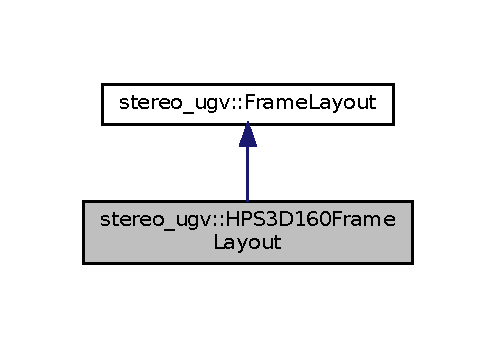
\includegraphics[width=238pt]{classstereo__ugv_1_1HPS3D160FrameLayout__inherit__graph}
\end{center}
\end{figure}


Collaboration diagram for stereo\+\_\+ugv\+:\+:H\+P\+S3\+D160\+Frame\+Layout\+:\nopagebreak
\begin{figure}[H]
\begin{center}
\leavevmode
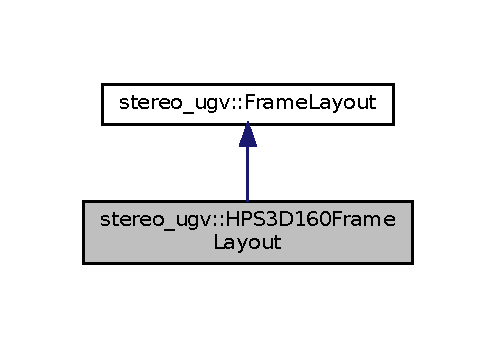
\includegraphics[width=238pt]{classstereo__ugv_1_1HPS3D160FrameLayout__coll__graph}
\end{center}
\end{figure}
\subsection*{Public Member Functions}
\begin{DoxyCompactItemize}
\item 
void \hyperlink{classstereo__ugv_1_1HPS3D160FrameLayout_af8ec41171a86b9ed3724d9e90b756fbb}{set\+Image\+Size} (cv\+::\+Size size)
\begin{DoxyCompactList}\small\item\em Sets the image size. \end{DoxyCompactList}\item 
virtual cv\+::\+Size \hyperlink{classstereo__ugv_1_1HPS3D160FrameLayout_add697132a4d32b0f1fc49f35f3b8fa0f}{frame\+Size} () const noexcept override
\begin{DoxyCompactList}\small\item\em Gets the frame size. \end{DoxyCompactList}\item 
virtual cv\+::\+Size \hyperlink{classstereo__ugv_1_1HPS3D160FrameLayout_ab7fb47261d8a8132ac0ca7a15b69500e}{image\+Size} () const noexcept override
\begin{DoxyCompactList}\small\item\em Gets the image size. The Stereo U\+GV package assumes that images taken by two heads of a stereo camera have the same size. \end{DoxyCompactList}\item 
virtual void \hyperlink{classstereo__ugv_1_1HPS3D160FrameLayout_a224d3fddea38c0c564baa8d391a396fa}{extract\+Images} (const cv\+::\+Mat \&frame, cv\+::\+Mat $\ast$left, cv\+::\+Mat $\ast$right) const override
\begin{DoxyCompactList}\small\item\em Extracts images from the given frame. The Stereo U\+GV package assumes that two heads of a stereo camera are aligned horizontally. \end{DoxyCompactList}\end{DoxyCompactItemize}
\subsection*{Additional Inherited Members}


\subsection{Detailed Description}
The class of frame layout for H\+P\+S-\/3\+D160 cameras. 

\subsection{Member Function Documentation}
\mbox{\Hypertarget{classstereo__ugv_1_1HPS3D160FrameLayout_a224d3fddea38c0c564baa8d391a396fa}\label{classstereo__ugv_1_1HPS3D160FrameLayout_a224d3fddea38c0c564baa8d391a396fa}} 
\index{stereo\+\_\+ugv\+::\+H\+P\+S3\+D160\+Frame\+Layout@{stereo\+\_\+ugv\+::\+H\+P\+S3\+D160\+Frame\+Layout}!extract\+Images@{extract\+Images}}
\index{extract\+Images@{extract\+Images}!stereo\+\_\+ugv\+::\+H\+P\+S3\+D160\+Frame\+Layout@{stereo\+\_\+ugv\+::\+H\+P\+S3\+D160\+Frame\+Layout}}
\subsubsection{\texorpdfstring{extract\+Images()}{extractImages()}}
{\footnotesize\ttfamily void stereo\+\_\+ugv\+::\+H\+P\+S3\+D160\+Frame\+Layout\+::extract\+Images (\begin{DoxyParamCaption}\item[{const cv\+::\+Mat \&}]{frame,  }\item[{cv\+::\+Mat $\ast$}]{left,  }\item[{cv\+::\+Mat $\ast$}]{right }\end{DoxyParamCaption}) const\hspace{0.3cm}{\ttfamily [override]}, {\ttfamily [virtual]}}



Extracts images from the given frame. The Stereo U\+GV package assumes that two heads of a stereo camera are aligned horizontally. 


\begin{DoxyParams}{Parameters}
{\em frame} & The frame. \\
\hline
{\em left} & The left image to be extracted. \\
\hline
{\em right} & The right image to be extracted. \\
\hline
\end{DoxyParams}


Implements \hyperlink{classstereo__ugv_1_1FrameLayout_af5ab49a35cfbb59a79863720e7985d29}{stereo\+\_\+ugv\+::\+Frame\+Layout}.

\mbox{\Hypertarget{classstereo__ugv_1_1HPS3D160FrameLayout_add697132a4d32b0f1fc49f35f3b8fa0f}\label{classstereo__ugv_1_1HPS3D160FrameLayout_add697132a4d32b0f1fc49f35f3b8fa0f}} 
\index{stereo\+\_\+ugv\+::\+H\+P\+S3\+D160\+Frame\+Layout@{stereo\+\_\+ugv\+::\+H\+P\+S3\+D160\+Frame\+Layout}!frame\+Size@{frame\+Size}}
\index{frame\+Size@{frame\+Size}!stereo\+\_\+ugv\+::\+H\+P\+S3\+D160\+Frame\+Layout@{stereo\+\_\+ugv\+::\+H\+P\+S3\+D160\+Frame\+Layout}}
\subsubsection{\texorpdfstring{frame\+Size()}{frameSize()}}
{\footnotesize\ttfamily cv\+::\+Size stereo\+\_\+ugv\+::\+H\+P\+S3\+D160\+Frame\+Layout\+::frame\+Size (\begin{DoxyParamCaption}{ }\end{DoxyParamCaption}) const\hspace{0.3cm}{\ttfamily [override]}, {\ttfamily [virtual]}, {\ttfamily [noexcept]}}



Gets the frame size. 

\begin{DoxyReturn}{Returns}
The frame size. 
\end{DoxyReturn}


Implements \hyperlink{classstereo__ugv_1_1FrameLayout_a59da4ac9d0cc6a43cccbf8666849bdc2}{stereo\+\_\+ugv\+::\+Frame\+Layout}.

\mbox{\Hypertarget{classstereo__ugv_1_1HPS3D160FrameLayout_ab7fb47261d8a8132ac0ca7a15b69500e}\label{classstereo__ugv_1_1HPS3D160FrameLayout_ab7fb47261d8a8132ac0ca7a15b69500e}} 
\index{stereo\+\_\+ugv\+::\+H\+P\+S3\+D160\+Frame\+Layout@{stereo\+\_\+ugv\+::\+H\+P\+S3\+D160\+Frame\+Layout}!image\+Size@{image\+Size}}
\index{image\+Size@{image\+Size}!stereo\+\_\+ugv\+::\+H\+P\+S3\+D160\+Frame\+Layout@{stereo\+\_\+ugv\+::\+H\+P\+S3\+D160\+Frame\+Layout}}
\subsubsection{\texorpdfstring{image\+Size()}{imageSize()}}
{\footnotesize\ttfamily cv\+::\+Size stereo\+\_\+ugv\+::\+H\+P\+S3\+D160\+Frame\+Layout\+::image\+Size (\begin{DoxyParamCaption}{ }\end{DoxyParamCaption}) const\hspace{0.3cm}{\ttfamily [override]}, {\ttfamily [virtual]}, {\ttfamily [noexcept]}}



Gets the image size. The Stereo U\+GV package assumes that images taken by two heads of a stereo camera have the same size. 

\begin{DoxyReturn}{Returns}
The image size. 
\end{DoxyReturn}


Implements \hyperlink{classstereo__ugv_1_1FrameLayout_a12cc36a89f8e66ffc6a2fa5eb3c5f648}{stereo\+\_\+ugv\+::\+Frame\+Layout}.

\mbox{\Hypertarget{classstereo__ugv_1_1HPS3D160FrameLayout_af8ec41171a86b9ed3724d9e90b756fbb}\label{classstereo__ugv_1_1HPS3D160FrameLayout_af8ec41171a86b9ed3724d9e90b756fbb}} 
\index{stereo\+\_\+ugv\+::\+H\+P\+S3\+D160\+Frame\+Layout@{stereo\+\_\+ugv\+::\+H\+P\+S3\+D160\+Frame\+Layout}!set\+Image\+Size@{set\+Image\+Size}}
\index{set\+Image\+Size@{set\+Image\+Size}!stereo\+\_\+ugv\+::\+H\+P\+S3\+D160\+Frame\+Layout@{stereo\+\_\+ugv\+::\+H\+P\+S3\+D160\+Frame\+Layout}}
\subsubsection{\texorpdfstring{set\+Image\+Size()}{setImageSize()}}
{\footnotesize\ttfamily void stereo\+\_\+ugv\+::\+H\+P\+S3\+D160\+Frame\+Layout\+::set\+Image\+Size (\begin{DoxyParamCaption}\item[{cv\+::\+Size}]{size }\end{DoxyParamCaption})}



Sets the image size. 


\begin{DoxyParams}{Parameters}
{\em size} & The image size. \\
\hline
\end{DoxyParams}


The documentation for this class was generated from the following files\+:\begin{DoxyCompactItemize}
\item 
/home/yunhao/stereo\+\_\+ugv/src/stereo\+\_\+ugv/include/stereo\+\_\+ugv/\hyperlink{frame__layout_8h}{frame\+\_\+layout.\+h}\item 
/home/yunhao/stereo\+\_\+ugv/src/stereo\+\_\+ugv/src/stereo\+\_\+ugv/frame\+\_\+layout.\+cpp\end{DoxyCompactItemize}

\hypertarget{classstereo__ugv_1_1ImageSource}{}\section{stereo\+\_\+ugv\+:\+:Image\+Source Class Reference}
\label{classstereo__ugv_1_1ImageSource}\index{stereo\+\_\+ugv\+::\+Image\+Source@{stereo\+\_\+ugv\+::\+Image\+Source}}


The base class that reads a pair of images taken by a stereo camera at a time from various sources.  




{\ttfamily \#include $<$image\+\_\+source.\+h$>$}



Inheritance diagram for stereo\+\_\+ugv\+:\+:Image\+Source\+:\nopagebreak
\begin{figure}[H]
\begin{center}
\leavevmode
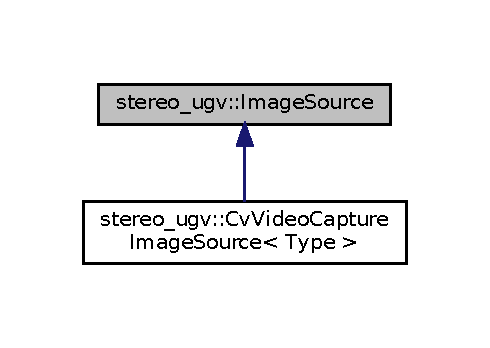
\includegraphics[width=235pt]{classstereo__ugv_1_1ImageSource__inherit__graph}
\end{center}
\end{figure}
\subsection*{Public Member Functions}
\begin{DoxyCompactItemize}
\item 
virtual cv\+::\+Size \hyperlink{classstereo__ugv_1_1ImageSource_a30d9146abcdcef11f03685a9887b96d0}{image\+Size} () const =0
\begin{DoxyCompactList}\small\item\em Gets the image size. The Stereo U\+GV package assumes that images taken by two heads of a stereo camera have the same size. \end{DoxyCompactList}\item 
virtual void \hyperlink{classstereo__ugv_1_1ImageSource_a3d87f7b09cd8889fcbee3efb29a0c39c}{read\+Images} (cv\+::\+Mat $\ast$left, cv\+::\+Mat $\ast$right)=0
\begin{DoxyCompactList}\small\item\em Reads a pair of images of the next frame. The Stereo U\+GV package assumes that two heads of a stereo camera are aligned horizontally. \end{DoxyCompactList}\end{DoxyCompactItemize}
\subsection*{Static Public Member Functions}
\begin{DoxyCompactItemize}
\item 
static std\+::unique\+\_\+ptr$<$ \hyperlink{classstereo__ugv_1_1ImageSource}{Image\+Source} $>$ \hyperlink{classstereo__ugv_1_1ImageSource_a18a1a40c3b5d51788bf4c68a4186ca31}{create} (const \hyperlink{classstereo__ugv_1_1Context}{Context} \&context)
\begin{DoxyCompactList}\small\item\em Creates an \hyperlink{classstereo__ugv_1_1ImageSource}{Image\+Source}. \end{DoxyCompactList}\end{DoxyCompactItemize}


\subsection{Detailed Description}
The base class that reads a pair of images taken by a stereo camera at a time from various sources. 

\subsection{Member Function Documentation}
\mbox{\Hypertarget{classstereo__ugv_1_1ImageSource_a18a1a40c3b5d51788bf4c68a4186ca31}\label{classstereo__ugv_1_1ImageSource_a18a1a40c3b5d51788bf4c68a4186ca31}} 
\index{stereo\+\_\+ugv\+::\+Image\+Source@{stereo\+\_\+ugv\+::\+Image\+Source}!create@{create}}
\index{create@{create}!stereo\+\_\+ugv\+::\+Image\+Source@{stereo\+\_\+ugv\+::\+Image\+Source}}
\subsubsection{\texorpdfstring{create()}{create()}}
{\footnotesize\ttfamily std\+::unique\+\_\+ptr$<$ \hyperlink{classstereo__ugv_1_1ImageSource}{Image\+Source} $>$ stereo\+\_\+ugv\+::\+Image\+Source\+::create (\begin{DoxyParamCaption}\item[{const \hyperlink{classstereo__ugv_1_1Context}{Context} \&}]{context }\end{DoxyParamCaption})\hspace{0.3cm}{\ttfamily [static]}}



Creates an \hyperlink{classstereo__ugv_1_1ImageSource}{Image\+Source}. 

The function determines the concrete subclass of the layout to be created by looking up the \char`\"{}type\char`\"{} key, and calls the corresponding initialization function. Currently, \char`\"{}camera\char`\"{}, \char`\"{}images\char`\"{} and \char`\"{}video\char`\"{} are supported. 
\begin{DoxyParams}{Parameters}
{\em context} & The context containing initialization parameters. \\
\hline
\end{DoxyParams}
\begin{DoxyReturn}{Returns}
A unique pointer to the created image source. 
\end{DoxyReturn}
\mbox{\Hypertarget{classstereo__ugv_1_1ImageSource_a30d9146abcdcef11f03685a9887b96d0}\label{classstereo__ugv_1_1ImageSource_a30d9146abcdcef11f03685a9887b96d0}} 
\index{stereo\+\_\+ugv\+::\+Image\+Source@{stereo\+\_\+ugv\+::\+Image\+Source}!image\+Size@{image\+Size}}
\index{image\+Size@{image\+Size}!stereo\+\_\+ugv\+::\+Image\+Source@{stereo\+\_\+ugv\+::\+Image\+Source}}
\subsubsection{\texorpdfstring{image\+Size()}{imageSize()}}
{\footnotesize\ttfamily virtual cv\+::\+Size stereo\+\_\+ugv\+::\+Image\+Source\+::image\+Size (\begin{DoxyParamCaption}{ }\end{DoxyParamCaption}) const\hspace{0.3cm}{\ttfamily [pure virtual]}}



Gets the image size. The Stereo U\+GV package assumes that images taken by two heads of a stereo camera have the same size. 

\begin{DoxyReturn}{Returns}
The image size. 
\end{DoxyReturn}


Implemented in \hyperlink{classstereo__ugv_1_1CvVideoCaptureImageSource_a84dd7dbd0ff6091d68843ca02a18e0cc}{stereo\+\_\+ugv\+::\+Cv\+Video\+Capture\+Image\+Source$<$ Type $>$}.

\mbox{\Hypertarget{classstereo__ugv_1_1ImageSource_a3d87f7b09cd8889fcbee3efb29a0c39c}\label{classstereo__ugv_1_1ImageSource_a3d87f7b09cd8889fcbee3efb29a0c39c}} 
\index{stereo\+\_\+ugv\+::\+Image\+Source@{stereo\+\_\+ugv\+::\+Image\+Source}!read\+Images@{read\+Images}}
\index{read\+Images@{read\+Images}!stereo\+\_\+ugv\+::\+Image\+Source@{stereo\+\_\+ugv\+::\+Image\+Source}}
\subsubsection{\texorpdfstring{read\+Images()}{readImages()}}
{\footnotesize\ttfamily virtual void stereo\+\_\+ugv\+::\+Image\+Source\+::read\+Images (\begin{DoxyParamCaption}\item[{cv\+::\+Mat $\ast$}]{left,  }\item[{cv\+::\+Mat $\ast$}]{right }\end{DoxyParamCaption})\hspace{0.3cm}{\ttfamily [pure virtual]}}



Reads a pair of images of the next frame. The Stereo U\+GV package assumes that two heads of a stereo camera are aligned horizontally. 


\begin{DoxyParams}{Parameters}
{\em left} & The image taken by the left head. \\
\hline
{\em right} & The image taken by the right head. \\
\hline
\end{DoxyParams}


Implemented in \hyperlink{classstereo__ugv_1_1CvVideoCaptureImageSource_a6636c97811bb28d59453c3865b0bda69}{stereo\+\_\+ugv\+::\+Cv\+Video\+Capture\+Image\+Source$<$ Type $>$}.



The documentation for this class was generated from the following files\+:\begin{DoxyCompactItemize}
\item 
/home/yunhao/stereo\+\_\+ugv/src/stereo\+\_\+ugv/include/stereo\+\_\+ugv/\hyperlink{image__source_8h}{image\+\_\+source.\+h}\item 
/home/yunhao/stereo\+\_\+ugv/src/stereo\+\_\+ugv/src/stereo\+\_\+ugv/image\+\_\+source.\+cpp\end{DoxyCompactItemize}

\hypertarget{classstereo__ugv_1_1InvalidParameter}{}\section{stereo\+\_\+ugv\+:\+:Invalid\+Parameter Class Reference}
\label{classstereo__ugv_1_1InvalidParameter}\index{stereo\+\_\+ugv\+::\+Invalid\+Parameter@{stereo\+\_\+ugv\+::\+Invalid\+Parameter}}


The class for errors due to unaccepted initialization parameters.  




{\ttfamily \#include $<$exception.\+h$>$}



Inheritance diagram for stereo\+\_\+ugv\+:\+:Invalid\+Parameter\+:
\nopagebreak
\begin{figure}[H]
\begin{center}
\leavevmode
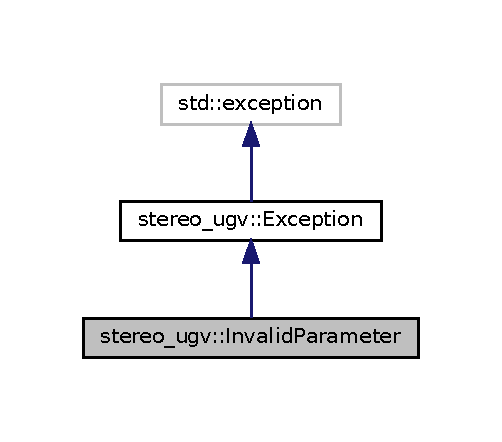
\includegraphics[width=241pt]{classstereo__ugv_1_1InvalidParameter__inherit__graph}
\end{center}
\end{figure}


Collaboration diagram for stereo\+\_\+ugv\+:\+:Invalid\+Parameter\+:
\nopagebreak
\begin{figure}[H]
\begin{center}
\leavevmode
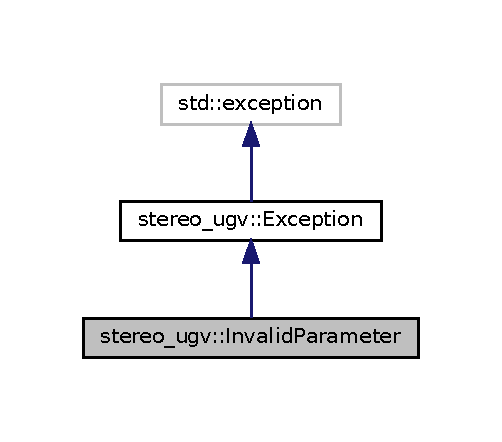
\includegraphics[width=241pt]{classstereo__ugv_1_1InvalidParameter__coll__graph}
\end{center}
\end{figure}
\subsection*{Additional Inherited Members}


\subsection{Detailed Description}
The class for errors due to unaccepted initialization parameters. 

The documentation for this class was generated from the following file\+:\begin{DoxyCompactItemize}
\item 
/home/yunhao/stereo\+\_\+ugv/src/stereo\+\_\+ugv/include/stereo\+\_\+ugv/\hyperlink{exception_8h}{exception.\+h}\end{DoxyCompactItemize}

\hypertarget{classstereo__ugv_1_1LensCalibrator}{}\section{stereo\+\_\+ugv\+:\+:Lens\+Calibrator Class Reference}
\label{classstereo__ugv_1_1LensCalibrator}\index{stereo\+\_\+ugv\+::\+Lens\+Calibrator@{stereo\+\_\+ugv\+::\+Lens\+Calibrator}}


The base class for calculating and saving undistortion coefficients of a stereo camera.  




{\ttfamily \#include $<$lens\+\_\+calibrator.\+h$>$}



Inheritance diagram for stereo\+\_\+ugv\+:\+:Lens\+Calibrator\+:
\nopagebreak
\begin{figure}[H]
\begin{center}
\leavevmode
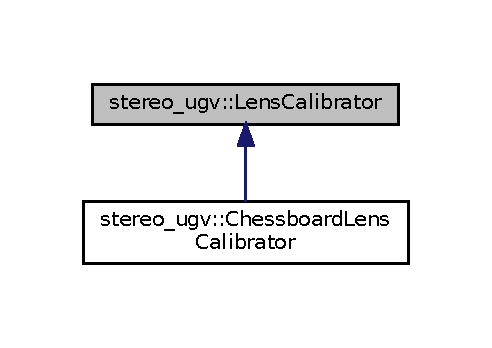
\includegraphics[width=236pt]{classstereo__ugv_1_1LensCalibrator__inherit__graph}
\end{center}
\end{figure}
\subsection*{Public Member Functions}
\begin{DoxyCompactItemize}
\item 
const \hyperlink{structstereo__ugv_1_1LensCoefficients}{Lens\+Coefficients} \& \hyperlink{classstereo__ugv_1_1LensCalibrator_a570522d1aa54e4ec153b47f6b86063e2}{coefficients} () const noexcept
\begin{DoxyCompactList}\small\item\em Gets the undistortion coefficients calculated by \hyperlink{classstereo__ugv_1_1LensCalibrator_aeeb532144b29ae7004ee14e2695def97}{calculate\+Coefficients()}. \end{DoxyCompactList}\item 
void \hyperlink{classstereo__ugv_1_1LensCalibrator_a13c279f4c0a4cc7b815340e31d5447be}{set\+Image\+Source} (std\+::unique\+\_\+ptr$<$ \hyperlink{classstereo__ugv_1_1ImageSource}{Image\+Source} $>$ \&\&source)
\begin{DoxyCompactList}\small\item\em Sets the image source. \end{DoxyCompactList}\item 
void \hyperlink{classstereo__ugv_1_1LensCalibrator_a8171c3a541429bd25ed64eb5140bbf2c}{set\+Max\+Image\+Count} (std\+::size\+\_\+t count)
\begin{DoxyCompactList}\small\item\em Sets the maximum number of image pairs used for calibration. \end{DoxyCompactList}\item 
void \hyperlink{classstereo__ugv_1_1LensCalibrator_a4debdb4b31e7b474576269cc15da15d7}{set\+Undistortion\+Filename} (std\+::string filename)
\begin{DoxyCompactList}\small\item\em The filename to which the calculated undistortion coefficients are written. \end{DoxyCompactList}\item 
\mbox{\Hypertarget{classstereo__ugv_1_1LensCalibrator_aeeb532144b29ae7004ee14e2695def97}\label{classstereo__ugv_1_1LensCalibrator_aeeb532144b29ae7004ee14e2695def97}} 
void \hyperlink{classstereo__ugv_1_1LensCalibrator_aeeb532144b29ae7004ee14e2695def97}{calculate\+Coefficients} ()
\begin{DoxyCompactList}\small\item\em Calculates the undistortion coefficients of the stereo camera and stores them in the internal \hyperlink{structstereo__ugv_1_1LensCoefficients}{Lens\+Coefficients}. \end{DoxyCompactList}\item 
\mbox{\Hypertarget{classstereo__ugv_1_1LensCalibrator_a770bc3091deec850b75b72d11ee9bda7}\label{classstereo__ugv_1_1LensCalibrator_a770bc3091deec850b75b72d11ee9bda7}} 
void \hyperlink{classstereo__ugv_1_1LensCalibrator_a770bc3091deec850b75b72d11ee9bda7}{save\+Coefficients} ()
\begin{DoxyCompactList}\small\item\em Saves the undistortion coefficients calculated by \hyperlink{classstereo__ugv_1_1LensCalibrator_aeeb532144b29ae7004ee14e2695def97}{calculate\+Coefficients()} into a Y\+A\+ML or X\+ML file whose name is specified by \hyperlink{classstereo__ugv_1_1LensCalibrator_a4debdb4b31e7b474576269cc15da15d7}{set\+Undistortion\+Filename()}. \end{DoxyCompactList}\end{DoxyCompactItemize}
\subsection*{Static Public Member Functions}
\begin{DoxyCompactItemize}
\item 
static std\+::unique\+\_\+ptr$<$ \hyperlink{classstereo__ugv_1_1LensCalibrator}{Lens\+Calibrator} $>$ \hyperlink{classstereo__ugv_1_1LensCalibrator_ae19b071e8cb8c015351d4717f79f9184}{create} (const \hyperlink{classstereo__ugv_1_1Context}{Context} \&context)
\begin{DoxyCompactList}\small\item\em Creates a \hyperlink{classstereo__ugv_1_1LensCalibrator}{Lens\+Calibrator}. \end{DoxyCompactList}\end{DoxyCompactItemize}
\subsection*{Protected Member Functions}
\begin{DoxyCompactItemize}
\item 
virtual bool \hyperlink{classstereo__ugv_1_1LensCalibrator_a9be834b0ef2983af47ac5f9dd67887fe}{detect\+Image\+Points} (const cv\+::\+Mat \&image, std\+::vector$<$ cv\+::\+Point2f $>$ $\ast$points) const =0
\begin{DoxyCompactList}\small\item\em Detects feature points in the given image. \end{DoxyCompactList}\item 
virtual std\+::vector$<$ cv\+::\+Point3f $>$ \hyperlink{classstereo__ugv_1_1LensCalibrator_a3edf81dfc9567904a0d1a7c3555d65bf}{create\+Object\+Points} () const =0
\begin{DoxyCompactList}\small\item\em Creates the 3D points corresponding to the detected 2D points in images. \end{DoxyCompactList}\item 
virtual int \hyperlink{classstereo__ugv_1_1LensCalibrator_ad25267d7b60a912f270701359eda1c54}{index\+Of\+Fixed\+Point} () const =0
\begin{DoxyCompactList}\small\item\em Gets the index of the fixed point if the method of releasing object is used. \end{DoxyCompactList}\end{DoxyCompactItemize}


\subsection{Detailed Description}
The base class for calculating and saving undistortion coefficients of a stereo camera. 

\subsection{Member Function Documentation}
\mbox{\Hypertarget{classstereo__ugv_1_1LensCalibrator_a570522d1aa54e4ec153b47f6b86063e2}\label{classstereo__ugv_1_1LensCalibrator_a570522d1aa54e4ec153b47f6b86063e2}} 
\index{stereo\+\_\+ugv\+::\+Lens\+Calibrator@{stereo\+\_\+ugv\+::\+Lens\+Calibrator}!coefficients@{coefficients}}
\index{coefficients@{coefficients}!stereo\+\_\+ugv\+::\+Lens\+Calibrator@{stereo\+\_\+ugv\+::\+Lens\+Calibrator}}
\subsubsection{\texorpdfstring{coefficients()}{coefficients()}}
{\footnotesize\ttfamily const \hyperlink{structstereo__ugv_1_1LensCoefficients}{Lens\+Coefficients} \& stereo\+\_\+ugv\+::\+Lens\+Calibrator\+::coefficients (\begin{DoxyParamCaption}{ }\end{DoxyParamCaption}) const\hspace{0.3cm}{\ttfamily [noexcept]}}



Gets the undistortion coefficients calculated by \hyperlink{classstereo__ugv_1_1LensCalibrator_aeeb532144b29ae7004ee14e2695def97}{calculate\+Coefficients()}. 

\begin{DoxyReturn}{Returns}
The undistortion coefficients. 
\end{DoxyReturn}
\mbox{\Hypertarget{classstereo__ugv_1_1LensCalibrator_ae19b071e8cb8c015351d4717f79f9184}\label{classstereo__ugv_1_1LensCalibrator_ae19b071e8cb8c015351d4717f79f9184}} 
\index{stereo\+\_\+ugv\+::\+Lens\+Calibrator@{stereo\+\_\+ugv\+::\+Lens\+Calibrator}!create@{create}}
\index{create@{create}!stereo\+\_\+ugv\+::\+Lens\+Calibrator@{stereo\+\_\+ugv\+::\+Lens\+Calibrator}}
\subsubsection{\texorpdfstring{create()}{create()}}
{\footnotesize\ttfamily std\+::unique\+\_\+ptr$<$ \hyperlink{classstereo__ugv_1_1LensCalibrator}{Lens\+Calibrator} $>$ stereo\+\_\+ugv\+::\+Lens\+Calibrator\+::create (\begin{DoxyParamCaption}\item[{const \hyperlink{classstereo__ugv_1_1Context}{Context} \&}]{context }\end{DoxyParamCaption})\hspace{0.3cm}{\ttfamily [static]}}



Creates a \hyperlink{classstereo__ugv_1_1LensCalibrator}{Lens\+Calibrator}. 

The function determines the concrete subclass of the lens calibrator to be created by looking up the \char`\"{}type\char`\"{} key, and calls the corresponding initialization function. Currently, only \char`\"{}chessboard\char`\"{} is supported. 
\begin{DoxyParams}{Parameters}
{\em context} & The context containing initialization parameters. \\
\hline
\end{DoxyParams}
\begin{DoxyReturn}{Returns}
A unique pointer to the created lens calibrator. 
\end{DoxyReturn}
\mbox{\Hypertarget{classstereo__ugv_1_1LensCalibrator_a3edf81dfc9567904a0d1a7c3555d65bf}\label{classstereo__ugv_1_1LensCalibrator_a3edf81dfc9567904a0d1a7c3555d65bf}} 
\index{stereo\+\_\+ugv\+::\+Lens\+Calibrator@{stereo\+\_\+ugv\+::\+Lens\+Calibrator}!create\+Object\+Points@{create\+Object\+Points}}
\index{create\+Object\+Points@{create\+Object\+Points}!stereo\+\_\+ugv\+::\+Lens\+Calibrator@{stereo\+\_\+ugv\+::\+Lens\+Calibrator}}
\subsubsection{\texorpdfstring{create\+Object\+Points()}{createObjectPoints()}}
{\footnotesize\ttfamily virtual std\+::vector$<$cv\+::\+Point3f$>$ stereo\+\_\+ugv\+::\+Lens\+Calibrator\+::create\+Object\+Points (\begin{DoxyParamCaption}{ }\end{DoxyParamCaption}) const\hspace{0.3cm}{\ttfamily [protected]}, {\ttfamily [pure virtual]}}



Creates the 3D points corresponding to the detected 2D points in images. 

\begin{DoxyReturn}{Returns}
A vector of 3D points. 
\end{DoxyReturn}


Implemented in \hyperlink{classstereo__ugv_1_1ChessboardLensCalibrator_adaeaa9e0a3203872ea8e5ef5b3482f7e}{stereo\+\_\+ugv\+::\+Chessboard\+Lens\+Calibrator}.

\mbox{\Hypertarget{classstereo__ugv_1_1LensCalibrator_a9be834b0ef2983af47ac5f9dd67887fe}\label{classstereo__ugv_1_1LensCalibrator_a9be834b0ef2983af47ac5f9dd67887fe}} 
\index{stereo\+\_\+ugv\+::\+Lens\+Calibrator@{stereo\+\_\+ugv\+::\+Lens\+Calibrator}!detect\+Image\+Points@{detect\+Image\+Points}}
\index{detect\+Image\+Points@{detect\+Image\+Points}!stereo\+\_\+ugv\+::\+Lens\+Calibrator@{stereo\+\_\+ugv\+::\+Lens\+Calibrator}}
\subsubsection{\texorpdfstring{detect\+Image\+Points()}{detectImagePoints()}}
{\footnotesize\ttfamily virtual bool stereo\+\_\+ugv\+::\+Lens\+Calibrator\+::detect\+Image\+Points (\begin{DoxyParamCaption}\item[{const cv\+::\+Mat \&}]{image,  }\item[{std\+::vector$<$ cv\+::\+Point2f $>$ $\ast$}]{points }\end{DoxyParamCaption}) const\hspace{0.3cm}{\ttfamily [protected]}, {\ttfamily [pure virtual]}}



Detects feature points in the given image. 

The number of detected points must be constant, and these 2D points should corresponds to fixed points on a roughly planar rigid body in 3D space. 
\begin{DoxyParams}{Parameters}
{\em image} & The image. \\
\hline
{\em points} & The feature points to be detected. It will not be assigned if no feature points were detected. \\
\hline
\end{DoxyParams}
\begin{DoxyReturn}{Returns}
Whether feature points are detected. 
\end{DoxyReturn}


Implemented in \hyperlink{classstereo__ugv_1_1ChessboardLensCalibrator_ac6e93519a72d4218bcb1f9a49a9c22eb}{stereo\+\_\+ugv\+::\+Chessboard\+Lens\+Calibrator}.

\mbox{\Hypertarget{classstereo__ugv_1_1LensCalibrator_ad25267d7b60a912f270701359eda1c54}\label{classstereo__ugv_1_1LensCalibrator_ad25267d7b60a912f270701359eda1c54}} 
\index{stereo\+\_\+ugv\+::\+Lens\+Calibrator@{stereo\+\_\+ugv\+::\+Lens\+Calibrator}!index\+Of\+Fixed\+Point@{index\+Of\+Fixed\+Point}}
\index{index\+Of\+Fixed\+Point@{index\+Of\+Fixed\+Point}!stereo\+\_\+ugv\+::\+Lens\+Calibrator@{stereo\+\_\+ugv\+::\+Lens\+Calibrator}}
\subsubsection{\texorpdfstring{index\+Of\+Fixed\+Point()}{indexOfFixedPoint()}}
{\footnotesize\ttfamily virtual int stereo\+\_\+ugv\+::\+Lens\+Calibrator\+::index\+Of\+Fixed\+Point (\begin{DoxyParamCaption}{ }\end{DoxyParamCaption}) const\hspace{0.3cm}{\ttfamily [protected]}, {\ttfamily [pure virtual]}}



Gets the index of the fixed point if the method of releasing object is used. 

\begin{DoxyReturn}{Returns}
If the traditional calibration method is used, returns 0. Otherwise if the method of releasing object is used, return the index of the fixed point which is between 1 and number\+\_\+of\+\_\+points -\/ 1. 
\end{DoxyReturn}


Implemented in \hyperlink{classstereo__ugv_1_1ChessboardLensCalibrator_a00aa88f3399b59ec686f6d506c73a910}{stereo\+\_\+ugv\+::\+Chessboard\+Lens\+Calibrator}.

\mbox{\Hypertarget{classstereo__ugv_1_1LensCalibrator_a13c279f4c0a4cc7b815340e31d5447be}\label{classstereo__ugv_1_1LensCalibrator_a13c279f4c0a4cc7b815340e31d5447be}} 
\index{stereo\+\_\+ugv\+::\+Lens\+Calibrator@{stereo\+\_\+ugv\+::\+Lens\+Calibrator}!set\+Image\+Source@{set\+Image\+Source}}
\index{set\+Image\+Source@{set\+Image\+Source}!stereo\+\_\+ugv\+::\+Lens\+Calibrator@{stereo\+\_\+ugv\+::\+Lens\+Calibrator}}
\subsubsection{\texorpdfstring{set\+Image\+Source()}{setImageSource()}}
{\footnotesize\ttfamily void stereo\+\_\+ugv\+::\+Lens\+Calibrator\+::set\+Image\+Source (\begin{DoxyParamCaption}\item[{std\+::unique\+\_\+ptr$<$ \hyperlink{classstereo__ugv_1_1ImageSource}{Image\+Source} $>$ \&\&}]{source }\end{DoxyParamCaption})}



Sets the image source. 


\begin{DoxyParams}{Parameters}
{\em source} & The image source. \\
\hline
\end{DoxyParams}
\mbox{\Hypertarget{classstereo__ugv_1_1LensCalibrator_a8171c3a541429bd25ed64eb5140bbf2c}\label{classstereo__ugv_1_1LensCalibrator_a8171c3a541429bd25ed64eb5140bbf2c}} 
\index{stereo\+\_\+ugv\+::\+Lens\+Calibrator@{stereo\+\_\+ugv\+::\+Lens\+Calibrator}!set\+Max\+Image\+Count@{set\+Max\+Image\+Count}}
\index{set\+Max\+Image\+Count@{set\+Max\+Image\+Count}!stereo\+\_\+ugv\+::\+Lens\+Calibrator@{stereo\+\_\+ugv\+::\+Lens\+Calibrator}}
\subsubsection{\texorpdfstring{set\+Max\+Image\+Count()}{setMaxImageCount()}}
{\footnotesize\ttfamily void stereo\+\_\+ugv\+::\+Lens\+Calibrator\+::set\+Max\+Image\+Count (\begin{DoxyParamCaption}\item[{std\+::size\+\_\+t}]{count }\end{DoxyParamCaption})}



Sets the maximum number of image pairs used for calibration. 


\begin{DoxyParams}{Parameters}
{\em count} & The maximum number of frames in which images taken by both heads have detected feature points. The calibrator will stop reading more images after reaching this limit. A zero value means there is no such limit. \\
\hline
\end{DoxyParams}
\mbox{\Hypertarget{classstereo__ugv_1_1LensCalibrator_a4debdb4b31e7b474576269cc15da15d7}\label{classstereo__ugv_1_1LensCalibrator_a4debdb4b31e7b474576269cc15da15d7}} 
\index{stereo\+\_\+ugv\+::\+Lens\+Calibrator@{stereo\+\_\+ugv\+::\+Lens\+Calibrator}!set\+Undistortion\+Filename@{set\+Undistortion\+Filename}}
\index{set\+Undistortion\+Filename@{set\+Undistortion\+Filename}!stereo\+\_\+ugv\+::\+Lens\+Calibrator@{stereo\+\_\+ugv\+::\+Lens\+Calibrator}}
\subsubsection{\texorpdfstring{set\+Undistortion\+Filename()}{setUndistortionFilename()}}
{\footnotesize\ttfamily void stereo\+\_\+ugv\+::\+Lens\+Calibrator\+::set\+Undistortion\+Filename (\begin{DoxyParamCaption}\item[{std\+::string}]{filename }\end{DoxyParamCaption})}



The filename to which the calculated undistortion coefficients are written. 


\begin{DoxyParams}{Parameters}
{\em filename} & The name of the undistortion file. \\
\hline
\end{DoxyParams}


The documentation for this class was generated from the following files\+:\begin{DoxyCompactItemize}
\item 
/home/yunhao/stereo\+\_\+ugv/src/stereo\+\_\+ugv/include/stereo\+\_\+ugv/\hyperlink{lens__calibrator_8h}{lens\+\_\+calibrator.\+h}\item 
/home/yunhao/stereo\+\_\+ugv/src/stereo\+\_\+ugv/src/stereo\+\_\+ugv/lens\+\_\+calibrator.\+cpp\end{DoxyCompactItemize}

\hypertarget{structstereo__ugv_1_1LensCoefficients}{}\section{stereo\+\_\+ugv\+:\+:Lens\+Coefficients Struct Reference}
\label{structstereo__ugv_1_1LensCoefficients}\index{stereo\+\_\+ugv\+::\+Lens\+Coefficients@{stereo\+\_\+ugv\+::\+Lens\+Coefficients}}


The structure of undistortion coefficients of a stereo camera.  




{\ttfamily \#include $<$lens\+\_\+calibrator.\+h$>$}

\subsection*{Public Attributes}
\begin{DoxyCompactItemize}
\item 
\mbox{\Hypertarget{structstereo__ugv_1_1LensCoefficients_a5508e7d6d3dc52cbe79451ab65673e2e}\label{structstereo__ugv_1_1LensCoefficients_a5508e7d6d3dc52cbe79451ab65673e2e}} 
cv\+::\+Mat \hyperlink{structstereo__ugv_1_1LensCoefficients_a5508e7d6d3dc52cbe79451ab65673e2e}{camera\+\_\+matrices} \mbox{[}2\mbox{]}
\begin{DoxyCompactList}\small\item\em 3x3 camera matrices of the left and the right heads, respectively. \end{DoxyCompactList}\item 
cv\+::\+Mat \hyperlink{structstereo__ugv_1_1LensCoefficients_a5fcc432a6c105509aaea4fe293a3352d}{distortion\+\_\+coefficients} \mbox{[}2\mbox{]}
\begin{DoxyCompactList}\small\item\em 5x1 distortion coefficients of the left and the right heads, respectively. \end{DoxyCompactList}\item 
\mbox{\Hypertarget{structstereo__ugv_1_1LensCoefficients_a659e8f3117f5dedea0fb74a4d6065f27}\label{structstereo__ugv_1_1LensCoefficients_a659e8f3117f5dedea0fb74a4d6065f27}} 
cv\+::\+Mat \hyperlink{structstereo__ugv_1_1LensCoefficients_a659e8f3117f5dedea0fb74a4d6065f27}{rotation\+\_\+matrix}
\begin{DoxyCompactList}\small\item\em The rotation matrix from the left head to the right head. \end{DoxyCompactList}\item 
\mbox{\Hypertarget{structstereo__ugv_1_1LensCoefficients_a60ab9feaa811aa39f62da750dd76f239}\label{structstereo__ugv_1_1LensCoefficients_a60ab9feaa811aa39f62da750dd76f239}} 
cv\+::\+Mat \hyperlink{structstereo__ugv_1_1LensCoefficients_a60ab9feaa811aa39f62da750dd76f239}{translation\+\_\+vector}
\begin{DoxyCompactList}\small\item\em The translation vector from the left head to the right head. \end{DoxyCompactList}\end{DoxyCompactItemize}


\subsection{Detailed Description}
The structure of undistortion coefficients of a stereo camera. 

\subsection{Member Data Documentation}
\mbox{\Hypertarget{structstereo__ugv_1_1LensCoefficients_a5fcc432a6c105509aaea4fe293a3352d}\label{structstereo__ugv_1_1LensCoefficients_a5fcc432a6c105509aaea4fe293a3352d}} 
\index{stereo\+\_\+ugv\+::\+Lens\+Coefficients@{stereo\+\_\+ugv\+::\+Lens\+Coefficients}!distortion\+\_\+coefficients@{distortion\+\_\+coefficients}}
\index{distortion\+\_\+coefficients@{distortion\+\_\+coefficients}!stereo\+\_\+ugv\+::\+Lens\+Coefficients@{stereo\+\_\+ugv\+::\+Lens\+Coefficients}}
\subsubsection{\texorpdfstring{distortion\+\_\+coefficients}{distortion\_coefficients}}
{\footnotesize\ttfamily cv\+::\+Mat stereo\+\_\+ugv\+::\+Lens\+Coefficients\+::distortion\+\_\+coefficients\mbox{[}2\mbox{]}}



5x1 distortion coefficients of the left and the right heads, respectively. 

The coefficients are ordered as (k1, k2, p1, p2, k3), where k describes radial distortions, and p describes tangential distortions. 

The documentation for this struct was generated from the following file\+:\begin{DoxyCompactItemize}
\item 
/home/yunhao/stereo\+\_\+ugv/src/stereo\+\_\+ugv/include/stereo\+\_\+ugv/\hyperlink{lens__calibrator_8h}{lens\+\_\+calibrator.\+h}\end{DoxyCompactItemize}

\hypertarget{classstereo__ugv_1_1OutOfFrames}{}\section{stereo\+\_\+ugv\+:\+:Out\+Of\+Frames Class Reference}
\label{classstereo__ugv_1_1OutOfFrames}\index{stereo\+\_\+ugv\+::\+Out\+Of\+Frames@{stereo\+\_\+ugv\+::\+Out\+Of\+Frames}}


The class of exception thrown when an image source is running out of frames.  




{\ttfamily \#include $<$exception.\+h$>$}



Inheritance diagram for stereo\+\_\+ugv\+:\+:Out\+Of\+Frames\+:\nopagebreak
\begin{figure}[H]
\begin{center}
\leavevmode
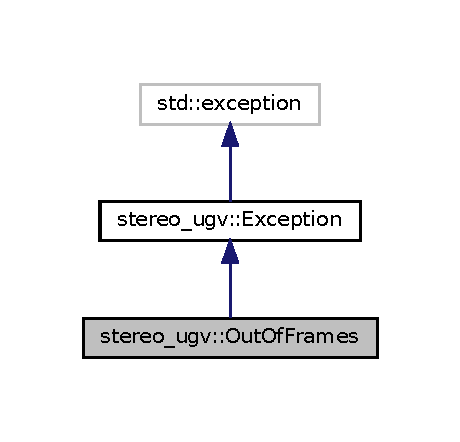
\includegraphics[width=221pt]{classstereo__ugv_1_1OutOfFrames__inherit__graph}
\end{center}
\end{figure}


Collaboration diagram for stereo\+\_\+ugv\+:\+:Out\+Of\+Frames\+:\nopagebreak
\begin{figure}[H]
\begin{center}
\leavevmode
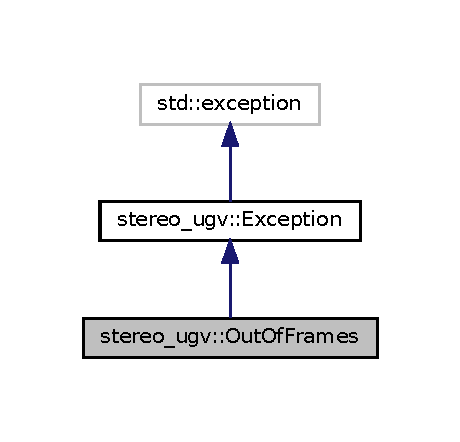
\includegraphics[width=221pt]{classstereo__ugv_1_1OutOfFrames__coll__graph}
\end{center}
\end{figure}
\subsection*{Additional Inherited Members}


\subsection{Detailed Description}
The class of exception thrown when an image source is running out of frames. 

The documentation for this class was generated from the following file\+:\begin{DoxyCompactItemize}
\item 
/home/yunhao/stereo\+\_\+ugv/src/stereo\+\_\+ugv/include/stereo\+\_\+ugv/\hyperlink{exception_8h}{exception.\+h}\end{DoxyCompactItemize}

\hypertarget{classstereo__ugv_1_1ParseError}{}\section{stereo\+\_\+ugv\+:\+:Parse\+Error Class Reference}
\label{classstereo__ugv_1_1ParseError}\index{stereo\+\_\+ugv\+::\+Parse\+Error@{stereo\+\_\+ugv\+::\+Parse\+Error}}


The class for parse errors encountered during variable substitution on strings within J\+S\+ON.  




{\ttfamily \#include $<$exception.\+h$>$}



Inheritance diagram for stereo\+\_\+ugv\+:\+:Parse\+Error\+:
\nopagebreak
\begin{figure}[H]
\begin{center}
\leavevmode
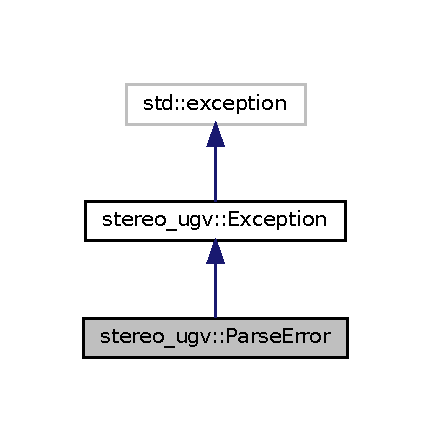
\includegraphics[width=207pt]{classstereo__ugv_1_1ParseError__inherit__graph}
\end{center}
\end{figure}


Collaboration diagram for stereo\+\_\+ugv\+:\+:Parse\+Error\+:
\nopagebreak
\begin{figure}[H]
\begin{center}
\leavevmode
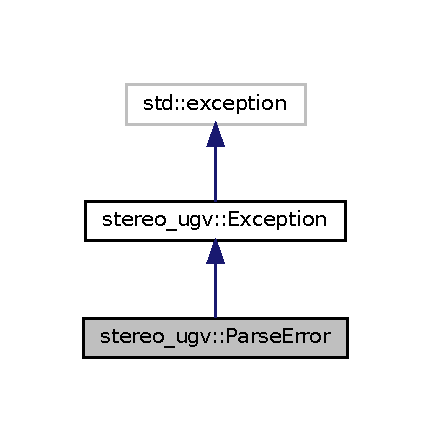
\includegraphics[width=207pt]{classstereo__ugv_1_1ParseError__coll__graph}
\end{center}
\end{figure}
\subsection*{Additional Inherited Members}


\subsection{Detailed Description}
The class for parse errors encountered during variable substitution on strings within J\+S\+ON. 

The documentation for this class was generated from the following file\+:\begin{DoxyCompactItemize}
\item 
/home/yunhao/stereo\+\_\+ugv/src/stereo\+\_\+ugv/include/stereo\+\_\+ugv/\hyperlink{exception_8h}{exception.\+h}\end{DoxyCompactItemize}

\hypertarget{classstereo__ugv_1_1RuntimeError}{}\section{stereo\+\_\+ugv\+:\+:Runtime\+Error Class Reference}
\label{classstereo__ugv_1_1RuntimeError}\index{stereo\+\_\+ugv\+::\+Runtime\+Error@{stereo\+\_\+ugv\+::\+Runtime\+Error}}


The class for errors that are not due to programming errors and do not have a clear cause.  




{\ttfamily \#include $<$exception.\+h$>$}



Inheritance diagram for stereo\+\_\+ugv\+:\+:Runtime\+Error\+:
\nopagebreak
\begin{figure}[H]
\begin{center}
\leavevmode
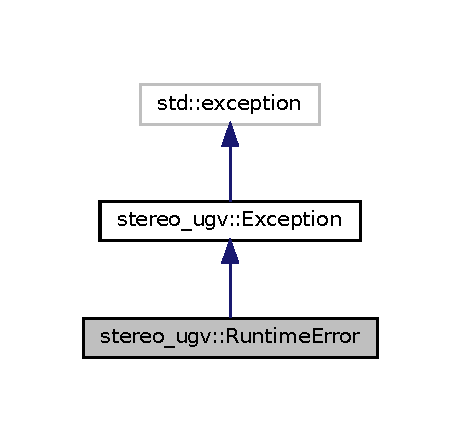
\includegraphics[width=221pt]{classstereo__ugv_1_1RuntimeError__inherit__graph}
\end{center}
\end{figure}


Collaboration diagram for stereo\+\_\+ugv\+:\+:Runtime\+Error\+:
\nopagebreak
\begin{figure}[H]
\begin{center}
\leavevmode
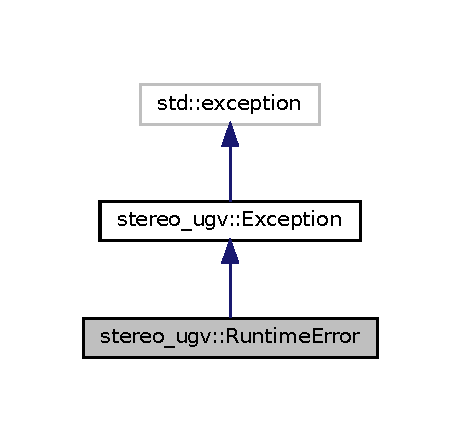
\includegraphics[width=221pt]{classstereo__ugv_1_1RuntimeError__coll__graph}
\end{center}
\end{figure}
\subsection*{Additional Inherited Members}


\subsection{Detailed Description}
The class for errors that are not due to programming errors and do not have a clear cause. 

The documentation for this class was generated from the following file\+:\begin{DoxyCompactItemize}
\item 
/home/yunhao/stereo\+\_\+ugv/src/stereo\+\_\+ugv/include/stereo\+\_\+ugv/\hyperlink{exception_8h}{exception.\+h}\end{DoxyCompactItemize}

\chapter{File Documentation}
\hypertarget{context_8h}{}\section{/home/yunhao/stereo\+\_\+ugv/src/stereo\+\_\+ugv/include/stereo\+\_\+ugv/context.h File Reference}
\label{context_8h}\index{/home/yunhao/stereo\+\_\+ugv/src/stereo\+\_\+ugv/include/stereo\+\_\+ugv/context.\+h@{/home/yunhao/stereo\+\_\+ugv/src/stereo\+\_\+ugv/include/stereo\+\_\+ugv/context.\+h}}


Defines \hyperlink{classstereo__ugv_1_1Context}{stereo\+\_\+ugv\+::\+Context} and initialization functions of several common types.  


{\ttfamily \#include $<$nlohmann/json.\+hpp$>$}\newline
{\ttfamily \#include $<$opencv2/core/types.\+hpp$>$}\newline
{\ttfamily \#include $<$image\+\_\+transport/image\+\_\+transport.\+h$>$}\newline
{\ttfamily \#include $<$ros/node\+\_\+handle.\+h$>$}\newline
{\ttfamily \#include $<$string$>$}\newline
{\ttfamily \#include $<$unordered\+\_\+map$>$}\newline
Include dependency graph for context.\+h\+:\nopagebreak
\begin{figure}[H]
\begin{center}
\leavevmode
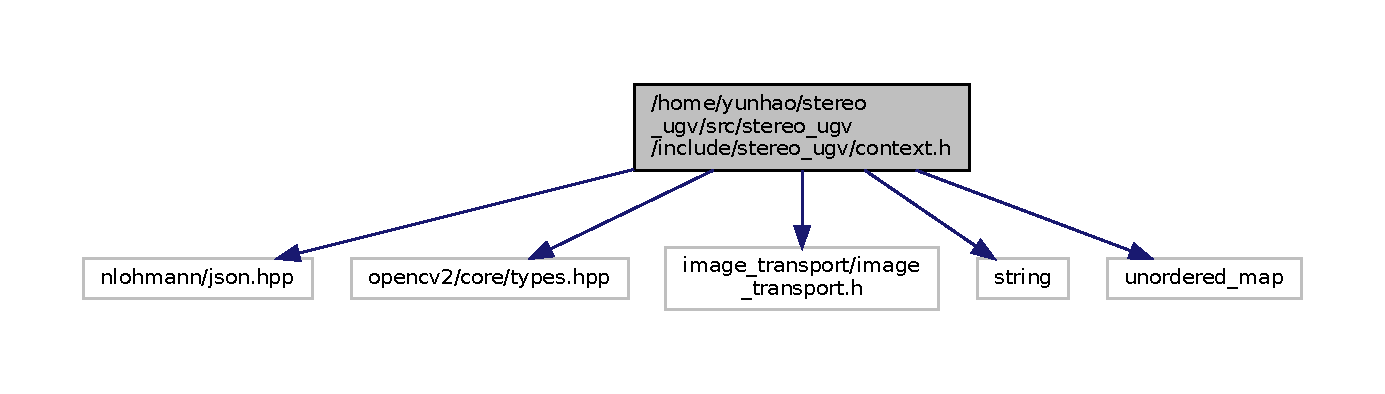
\includegraphics[width=350pt]{context_8h__incl}
\end{center}
\end{figure}
This graph shows which files directly or indirectly include this file\+:
\nopagebreak
\begin{figure}[H]
\begin{center}
\leavevmode
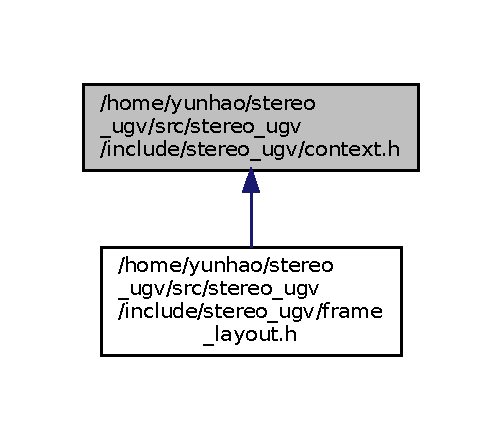
\includegraphics[width=241pt]{context_8h__dep__incl}
\end{center}
\end{figure}
\subsection*{Classes}
\begin{DoxyCompactItemize}
\item 
class \hyperlink{classstereo__ugv_1_1Context}{stereo\+\_\+ugv\+::\+Context}
\begin{DoxyCompactList}\small\item\em The class for initializing objects from parameters stored in J\+S\+ON files. \end{DoxyCompactList}\end{DoxyCompactItemize}
\subsection*{Namespaces}
\begin{DoxyCompactItemize}
\item 
 \hyperlink{namespacestereo__ugv}{stereo\+\_\+ugv}
\begin{DoxyCompactList}\small\item\em The namespace for public classes and functions of the Stereo U\+GV package. \end{DoxyCompactList}\end{DoxyCompactItemize}
\subsection*{Functions}
\begin{DoxyCompactItemize}
\item 
void \hyperlink{namespacestereo__ugv_a68c69a3de2a5351d41ce848792c213f4}{stereo\+\_\+ugv\+::initialize\+Context\+Arguments} (const ros\+::\+Node\+Handle \&node\+\_\+handle, nlohmann\+::json $\ast$parameter\+\_\+json, std\+::unordered\+\_\+map$<$ std\+::string, std\+::string $>$ $\ast$variable\+\_\+map)
\begin{DoxyCompactList}\small\item\em Initializes arguments to the \hyperlink{classstereo__ugv_1_1Context}{Context} constructor from parameters of a node handle. \end{DoxyCompactList}\item 
{\footnotesize template$<$typename T $>$ }\\void \hyperlink{namespacestereo__ugv_a6971cc11001fdf589a71f6fb3099c65b}{stereo\+\_\+ugv\+::initialize} (T $\ast$parameter, const Context \&context)
\begin{DoxyCompactList}\small\item\em Initializes a parameter. \end{DoxyCompactList}\item 
void \hyperlink{namespacestereo__ugv_aaa158ec1ee9178414843adbbb91a394b}{stereo\+\_\+ugv\+::initialize} (std\+::string $\ast$string, const Context \&context)
\begin{DoxyCompactList}\small\item\em Initializes an std\+::string and performs variable substitution. \end{DoxyCompactList}\item 
void \hyperlink{namespacestereo__ugv_adab204dc6f43824bcda4cd5e172d2812}{stereo\+\_\+ugv\+::initialize} (cv\+::\+Size $\ast$size, const Context \&context)
\begin{DoxyCompactList}\small\item\em Initializes a cv\+::\+Size. \end{DoxyCompactList}\item 
void \hyperlink{namespacestereo__ugv_a0a98148c84d1f085ac51c2f2fb7c8e7a}{stereo\+\_\+ugv\+::initialize} (cv\+::\+Term\+Criteria $\ast$criteria, const Context \&context)
\begin{DoxyCompactList}\small\item\em Initializes a cv\+::\+Term\+Criteria. \end{DoxyCompactList}\item 
Context \hyperlink{namespacestereo__ugv_aef8f9a951e11f9d5d178db99754aac4b}{stereo\+\_\+ugv\+::open\+Internal\+Context} (nlohmann\+::json $\ast$json, const Context \&context)
\begin{DoxyCompactList}\small\item\em Opens the internal context whose variable J\+S\+ON is stored in a separate file. \end{DoxyCompactList}\end{DoxyCompactItemize}


\subsection{Detailed Description}
Defines \hyperlink{classstereo__ugv_1_1Context}{stereo\+\_\+ugv\+::\+Context} and initialization functions of several common types. 


\hypertarget{exception_8h}{}\section{/home/yunhao/stereo\+\_\+ugv/src/stereo\+\_\+ugv/include/stereo\+\_\+ugv/exception.h File Reference}
\label{exception_8h}\index{/home/yunhao/stereo\+\_\+ugv/src/stereo\+\_\+ugv/include/stereo\+\_\+ugv/exception.\+h@{/home/yunhao/stereo\+\_\+ugv/src/stereo\+\_\+ugv/include/stereo\+\_\+ugv/exception.\+h}}


Defines \hyperlink{classstereo__ugv_1_1Exception}{stereo\+\_\+ugv\+::\+Exception} and its subclasses.  


{\ttfamily \#include $<$exception$>$}\newline
{\ttfamily \#include $<$memory$>$}\newline
{\ttfamily \#include $<$string$>$}\newline
Include dependency graph for exception.\+h\+:
\nopagebreak
\begin{figure}[H]
\begin{center}
\leavevmode
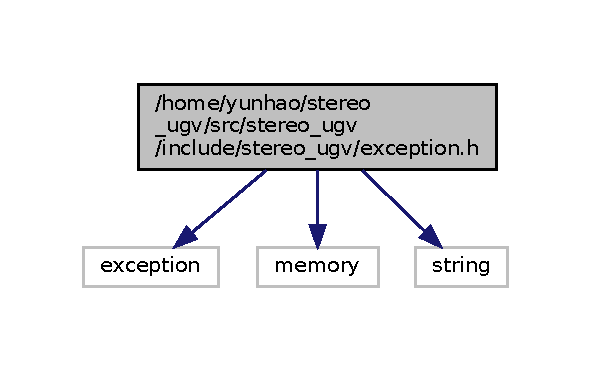
\includegraphics[width=284pt]{exception_8h__incl}
\end{center}
\end{figure}
This graph shows which files directly or indirectly include this file\+:
\nopagebreak
\begin{figure}[H]
\begin{center}
\leavevmode
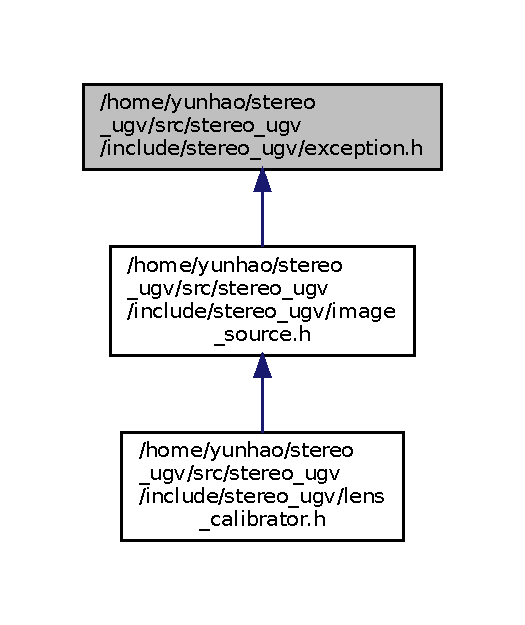
\includegraphics[width=252pt]{exception_8h__dep__incl}
\end{center}
\end{figure}
\subsection*{Classes}
\begin{DoxyCompactItemize}
\item 
class \hyperlink{classstereo__ugv_1_1Exception}{stereo\+\_\+ugv\+::\+Exception}
\begin{DoxyCompactList}\small\item\em The base class for exceptions. \end{DoxyCompactList}\item 
class \hyperlink{classstereo__ugv_1_1ParseError}{stereo\+\_\+ugv\+::\+Parse\+Error}
\begin{DoxyCompactList}\small\item\em The class for parse errors encountered during variable substitution on strings within J\+S\+ON. \end{DoxyCompactList}\item 
class \hyperlink{classstereo__ugv_1_1InvalidParameter}{stereo\+\_\+ugv\+::\+Invalid\+Parameter}
\begin{DoxyCompactList}\small\item\em The class for errors due to unaccepted initialization parameters. \end{DoxyCompactList}\item 
class \hyperlink{classstereo__ugv_1_1RuntimeError}{stereo\+\_\+ugv\+::\+Runtime\+Error}
\begin{DoxyCompactList}\small\item\em The class for errors that are not due to programming errors and do not have a clear cause. \end{DoxyCompactList}\item 
class \hyperlink{classstereo__ugv_1_1OutOfFrames}{stereo\+\_\+ugv\+::\+Out\+Of\+Frames}
\begin{DoxyCompactList}\small\item\em The class of exception thrown when an image source is running out of frames. \end{DoxyCompactList}\end{DoxyCompactItemize}
\subsection*{Namespaces}
\begin{DoxyCompactItemize}
\item 
 \hyperlink{namespacestereo__ugv}{stereo\+\_\+ugv}
\begin{DoxyCompactList}\small\item\em The namespace for public classes and functions of the \hyperlink{namespacestereo__ugv}{stereo\+\_\+ugv} package. \end{DoxyCompactList}\end{DoxyCompactItemize}
\subsection*{Macros}
\begin{DoxyCompactItemize}
\item 
\#define \hyperlink{exception_8h_a7f56c08588421dff58eeda23a2d41169}{S\+T\+E\+R\+E\+O\+\_\+\+U\+G\+V\+\_\+\+C\+H\+E\+C\+K\+\_\+\+P\+A\+R\+A\+M\+E\+T\+ER}(condition)
\begin{DoxyCompactList}\small\item\em Checks the validity of parameters by asserting that the given condition is true. Throws an Invalid\+Parameter if the assertion fails. \end{DoxyCompactList}\end{DoxyCompactItemize}


\subsection{Detailed Description}
Defines \hyperlink{classstereo__ugv_1_1Exception}{stereo\+\_\+ugv\+::\+Exception} and its subclasses. 



\subsection{Macro Definition Documentation}
\mbox{\Hypertarget{exception_8h_a7f56c08588421dff58eeda23a2d41169}\label{exception_8h_a7f56c08588421dff58eeda23a2d41169}} 
\index{exception.\+h@{exception.\+h}!S\+T\+E\+R\+E\+O\+\_\+\+U\+G\+V\+\_\+\+C\+H\+E\+C\+K\+\_\+\+P\+A\+R\+A\+M\+E\+T\+ER@{S\+T\+E\+R\+E\+O\+\_\+\+U\+G\+V\+\_\+\+C\+H\+E\+C\+K\+\_\+\+P\+A\+R\+A\+M\+E\+T\+ER}}
\index{S\+T\+E\+R\+E\+O\+\_\+\+U\+G\+V\+\_\+\+C\+H\+E\+C\+K\+\_\+\+P\+A\+R\+A\+M\+E\+T\+ER@{S\+T\+E\+R\+E\+O\+\_\+\+U\+G\+V\+\_\+\+C\+H\+E\+C\+K\+\_\+\+P\+A\+R\+A\+M\+E\+T\+ER}!exception.\+h@{exception.\+h}}
\subsubsection{\texorpdfstring{S\+T\+E\+R\+E\+O\+\_\+\+U\+G\+V\+\_\+\+C\+H\+E\+C\+K\+\_\+\+P\+A\+R\+A\+M\+E\+T\+ER}{STEREO\_UGV\_CHECK\_PARAMETER}}
{\footnotesize\ttfamily \#define S\+T\+E\+R\+E\+O\+\_\+\+U\+G\+V\+\_\+\+C\+H\+E\+C\+K\+\_\+\+P\+A\+R\+A\+M\+E\+T\+ER(\begin{DoxyParamCaption}\item[{}]{condition }\end{DoxyParamCaption})}

{\bfseries Value\+:}
\begin{DoxyCode}
\textcolor{keywordflow}{do}                                                                                                         
                \(\backslash\)
  \{                                                                                                        
                  \(\backslash\)
    if (!static\_cast<bool>(condition))                                                                     
                  \(\backslash\)
    \{                                                                                                      
                  \(\backslash\)
      throw \hyperlink{classstereo__ugv_1_1InvalidParameter}{stereo\_ugv::InvalidParameter}\{ \textcolor{stringliteral}{"Failed parameter check \(\backslash\)""} #
      condition \textcolor{stringliteral}{"\(\backslash\)""} \};                               \(\backslash\)
    \}                                                                                                      
                  \(\backslash\)
  \} \textcolor{keywordflow}{while} (\textcolor{keyword}{false})
\end{DoxyCode}


Checks the validity of parameters by asserting that the given condition is true. Throws an Invalid\+Parameter if the assertion fails. 


\begin{DoxyParams}{Parameters}
{\em condition} & A boolean expression that is supposed to be true. \\
\hline
\end{DoxyParams}

\hypertarget{frame__layout_8h}{}\section{/home/yunhao/stereo\+\_\+ugv/src/stereo\+\_\+ugv/include/stereo\+\_\+ugv/frame\+\_\+layout.h File Reference}
\label{frame__layout_8h}\index{/home/yunhao/stereo\+\_\+ugv/src/stereo\+\_\+ugv/include/stereo\+\_\+ugv/frame\+\_\+layout.\+h@{/home/yunhao/stereo\+\_\+ugv/src/stereo\+\_\+ugv/include/stereo\+\_\+ugv/frame\+\_\+layout.\+h}}


Defines \hyperlink{classstereo__ugv_1_1FrameLayout}{stereo\+\_\+ugv\+::\+Frame\+Layout} and its subclasses.  


{\ttfamily \#include \char`\"{}stereo\+\_\+ugv/context.\+h\char`\"{}}\newline
{\ttfamily \#include $<$opencv2/core/mat.\+hpp$>$}\newline
{\ttfamily \#include $<$memory$>$}\newline
Include dependency graph for frame\+\_\+layout.\+h\+:
\nopagebreak
\begin{figure}[H]
\begin{center}
\leavevmode
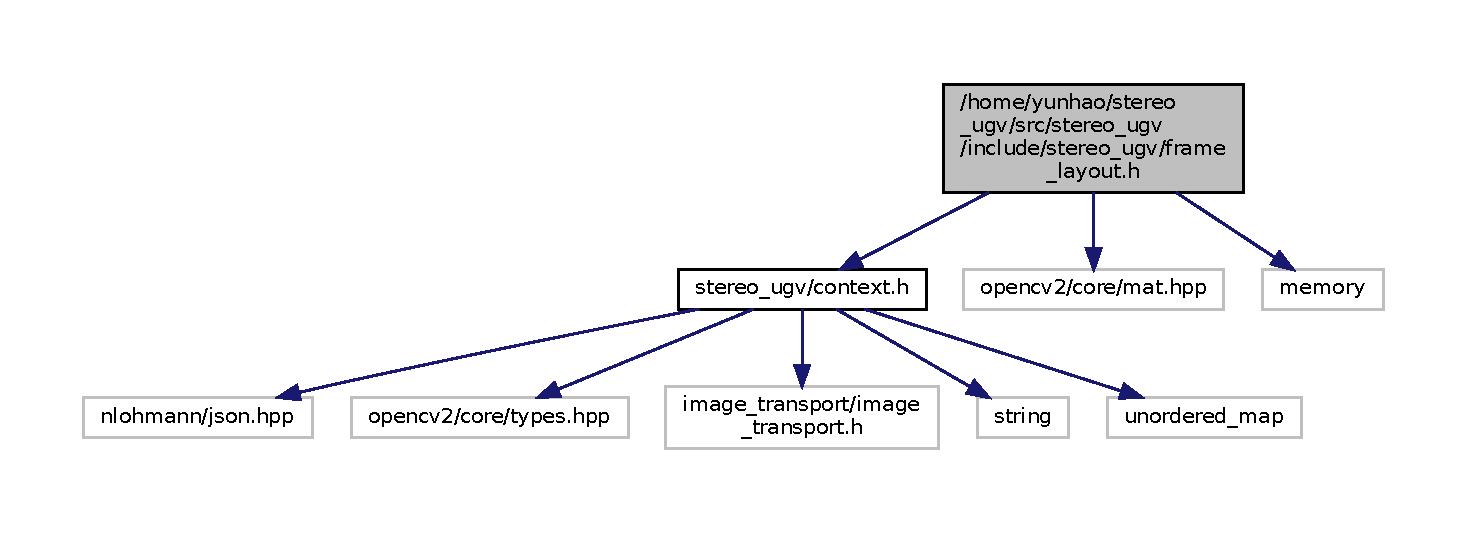
\includegraphics[width=350pt]{frame__layout_8h__incl}
\end{center}
\end{figure}
This graph shows which files directly or indirectly include this file\+:
\nopagebreak
\begin{figure}[H]
\begin{center}
\leavevmode
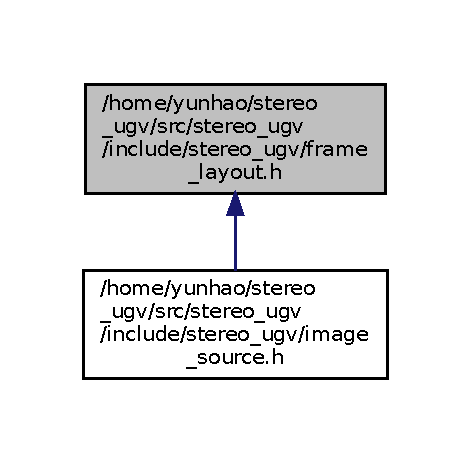
\includegraphics[width=226pt]{frame__layout_8h__dep__incl}
\end{center}
\end{figure}
\subsection*{Classes}
\begin{DoxyCompactItemize}
\item 
class \hyperlink{classstereo__ugv_1_1FrameLayout}{stereo\+\_\+ugv\+::\+Frame\+Layout}
\begin{DoxyCompactList}\small\item\em The base class that defines how images taken by two heads of a stereo camera are positioned in the same frame. \end{DoxyCompactList}\item 
class \hyperlink{classstereo__ugv_1_1HPS3D160FrameLayout}{stereo\+\_\+ugv\+::\+H\+P\+S3\+D160\+Frame\+Layout}
\begin{DoxyCompactList}\small\item\em The class of frame layout for H\+P\+S-\/3\+D160 cameras. \end{DoxyCompactList}\end{DoxyCompactItemize}
\subsection*{Namespaces}
\begin{DoxyCompactItemize}
\item 
 \hyperlink{namespacestereo__ugv}{stereo\+\_\+ugv}
\begin{DoxyCompactList}\small\item\em The namespace for public classes and functions of the Stereo U\+GV package. \end{DoxyCompactList}\end{DoxyCompactItemize}
\subsection*{Functions}
\begin{DoxyCompactItemize}
\item 
void \hyperlink{namespacestereo__ugv_ac02cc03581ba53b911a9a7bd87f9a24c}{stereo\+\_\+ugv\+::initialize} (H\+P\+S3\+D160\+Frame\+Layout $\ast$layout, const Context \&context)
\begin{DoxyCompactList}\small\item\em Initializes an \hyperlink{classstereo__ugv_1_1HPS3D160FrameLayout}{H\+P\+S3\+D160\+Frame\+Layout}. \end{DoxyCompactList}\end{DoxyCompactItemize}


\subsection{Detailed Description}
Defines \hyperlink{classstereo__ugv_1_1FrameLayout}{stereo\+\_\+ugv\+::\+Frame\+Layout} and its subclasses. 


\hypertarget{image__source_8h}{}\section{/home/yunhao/stereo\+\_\+ugv/src/stereo\+\_\+ugv/include/stereo\+\_\+ugv/image\+\_\+source.h File Reference}
\label{image__source_8h}\index{/home/yunhao/stereo\+\_\+ugv/src/stereo\+\_\+ugv/include/stereo\+\_\+ugv/image\+\_\+source.\+h@{/home/yunhao/stereo\+\_\+ugv/src/stereo\+\_\+ugv/include/stereo\+\_\+ugv/image\+\_\+source.\+h}}


Defines \hyperlink{classstereo__ugv_1_1ImageSource}{stereo\+\_\+ugv\+::\+Image\+Source} and its subclasses.  


{\ttfamily \#include \char`\"{}stereo\+\_\+ugv/exception.\+h\char`\"{}}\newline
{\ttfamily \#include \char`\"{}stereo\+\_\+ugv/frame\+\_\+layout.\+h\char`\"{}}\newline
{\ttfamily \#include $<$fmt/core.\+h$>$}\newline
{\ttfamily \#include $<$opencv2/videoio.\+hpp$>$}\newline
{\ttfamily \#include $<$ros/console.\+h$>$}\newline
{\ttfamily \#include $<$utility$>$}\newline
Include dependency graph for image\+\_\+source.\+h\+:
\nopagebreak
\begin{figure}[H]
\begin{center}
\leavevmode
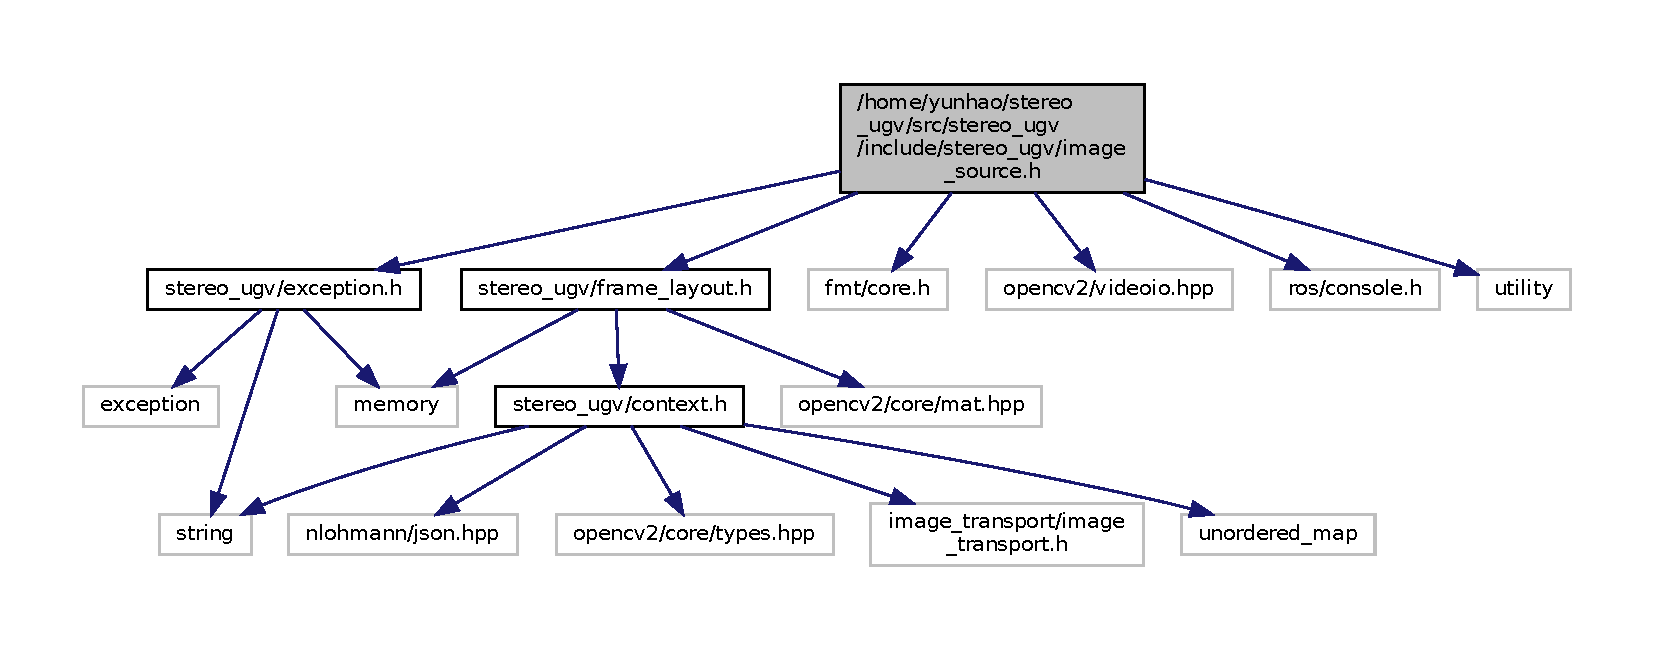
\includegraphics[width=350pt]{image__source_8h__incl}
\end{center}
\end{figure}
\subsection*{Classes}
\begin{DoxyCompactItemize}
\item 
class \hyperlink{classstereo__ugv_1_1ImageSource}{stereo\+\_\+ugv\+::\+Image\+Source}
\begin{DoxyCompactList}\small\item\em The base class that reads a pair of images taken by a stereo camera at a time from various sources. \end{DoxyCompactList}\item 
class \hyperlink{classstereo__ugv_1_1CvVideoCaptureImageSource}{stereo\+\_\+ugv\+::\+Cv\+Video\+Capture\+Image\+Source$<$ Type $>$}
\begin{DoxyCompactList}\small\item\em Class for image sources backended by cv\+::\+Video\+Capture. \end{DoxyCompactList}\end{DoxyCompactItemize}
\subsection*{Namespaces}
\begin{DoxyCompactItemize}
\item 
 \hyperlink{namespacestereo__ugv}{stereo\+\_\+ugv}
\begin{DoxyCompactList}\small\item\em The namespace for public classes and functions of the Stereo U\+GV package. \end{DoxyCompactList}\end{DoxyCompactItemize}
\subsection*{Enumerations}
\begin{DoxyCompactItemize}
\item 
enum \hyperlink{namespacestereo__ugv_a5c139e7cfac12e9270ca903f1ce2e4bc}{stereo\+\_\+ugv\+::\+Cv\+Video\+Capture\+Type} \{ \hyperlink{namespacestereo__ugv_a5c139e7cfac12e9270ca903f1ce2e4bcaddf0d6b21537d984fea6544f58101fa8}{stereo\+\_\+ugv\+::\+Cv\+Video\+Capture\+Type\+::\+C\+A\+M\+E\+RA}, 
\hyperlink{namespacestereo__ugv_a5c139e7cfac12e9270ca903f1ce2e4bcab34687a3607271050f02aa9bf90c731a}{stereo\+\_\+ugv\+::\+Cv\+Video\+Capture\+Type\+::\+I\+M\+A\+G\+ES}, 
\hyperlink{namespacestereo__ugv_a5c139e7cfac12e9270ca903f1ce2e4bcae60ae31f67ab883c746bb71c7a145c18}{stereo\+\_\+ugv\+::\+Cv\+Video\+Capture\+Type\+::\+V\+I\+D\+EO}
 \}\begin{DoxyCompactList}\small\item\em Types of image sources backended by cv\+::\+Video\+Capture. \end{DoxyCompactList}
\end{DoxyCompactItemize}
\subsection*{Functions}
\begin{DoxyCompactItemize}
\item 
std\+::string \hyperlink{namespacestereo__ugv_af45c67058883fb26e2c27945af6ab490}{stereo\+\_\+ugv\+::find\+Camera\+Character\+Device\+File} (const std\+::string \&)
\begin{DoxyCompactList}\small\item\em Finds the character device file of a camera device given the prefix of its device name. \end{DoxyCompactList}\item 
{\footnotesize template$<$Cv\+Video\+Capture\+Type Type$>$ }\\void \hyperlink{namespacestereo__ugv_acaec0936792769b5d676773f7d4070cd}{stereo\+\_\+ugv\+::initialize} (Cv\+Video\+Capture\+Image\+Source$<$ Type $>$ $\ast$source, const Context \&context)
\begin{DoxyCompactList}\small\item\em Initializes a Cv\+Video\+Capture\+Image\+Source$<$\+Type$>$. \end{DoxyCompactList}\end{DoxyCompactItemize}


\subsection{Detailed Description}
Defines \hyperlink{classstereo__ugv_1_1ImageSource}{stereo\+\_\+ugv\+::\+Image\+Source} and its subclasses. 


\hypertarget{lens__calibrator_8h}{}\section{/home/yunhao/stereo\+\_\+ugv/src/stereo\+\_\+ugv/include/stereo\+\_\+ugv/lens\+\_\+calibrator.h File Reference}
\label{lens__calibrator_8h}\index{/home/yunhao/stereo\+\_\+ugv/src/stereo\+\_\+ugv/include/stereo\+\_\+ugv/lens\+\_\+calibrator.\+h@{/home/yunhao/stereo\+\_\+ugv/src/stereo\+\_\+ugv/include/stereo\+\_\+ugv/lens\+\_\+calibrator.\+h}}


Defines \hyperlink{classstereo__ugv_1_1LensCalibrator}{stereo\+\_\+ugv\+::\+Lens\+Calibrator} and its subclasses.  


{\ttfamily \#include \char`\"{}image\+\_\+source.\+h\char`\"{}}\newline
{\ttfamily \#include $<$cstddef$>$}\newline
{\ttfamily \#include $<$vector$>$}\newline
Include dependency graph for lens\+\_\+calibrator.\+h\+:\nopagebreak
\begin{figure}[H]
\begin{center}
\leavevmode
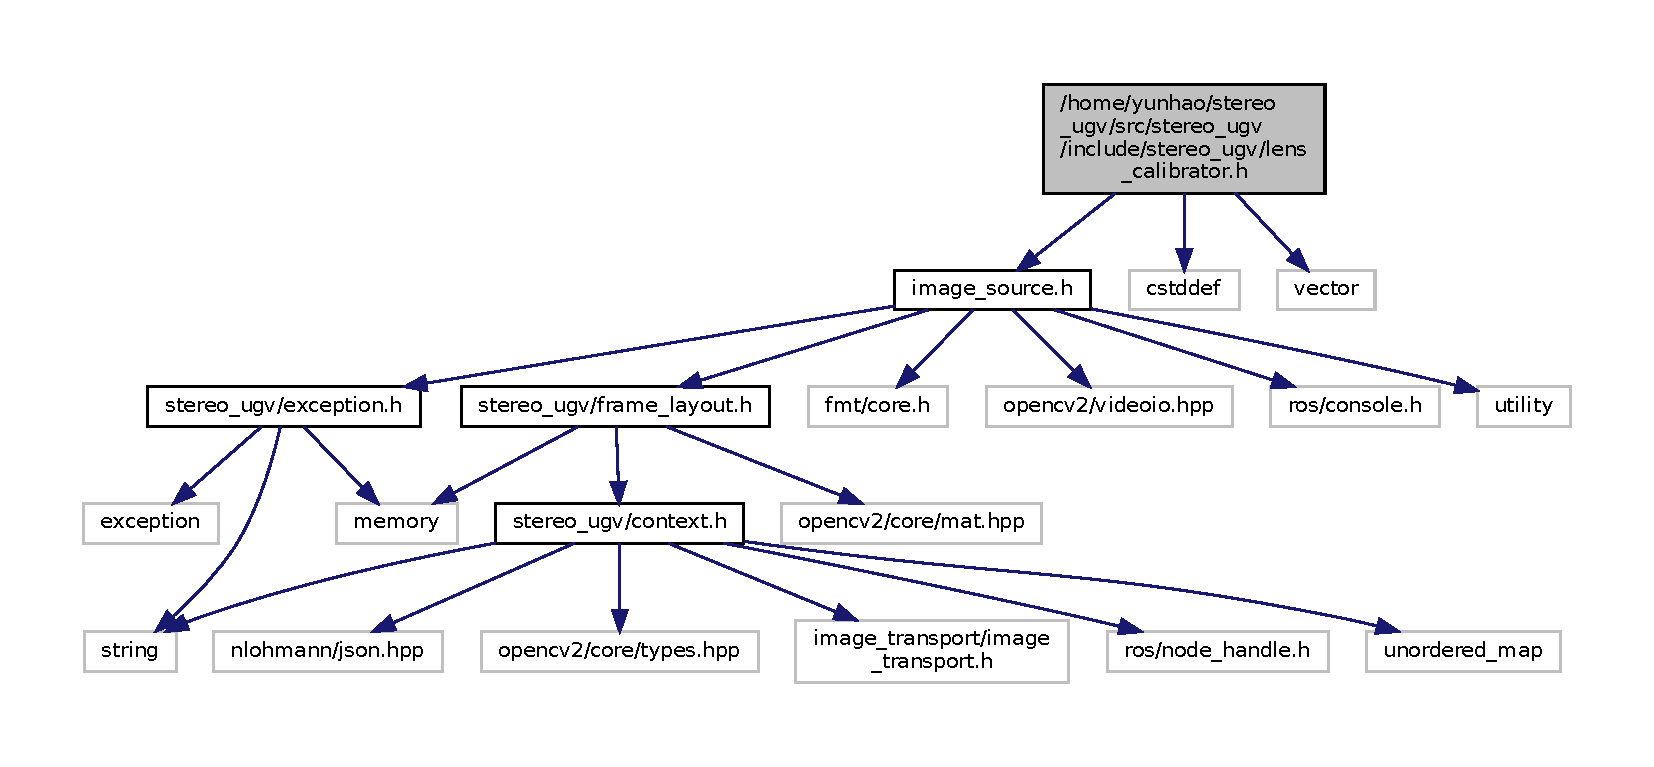
\includegraphics[width=350pt]{lens__calibrator_8h__incl}
\end{center}
\end{figure}
This graph shows which files directly or indirectly include this file\+:\nopagebreak
\begin{figure}[H]
\begin{center}
\leavevmode
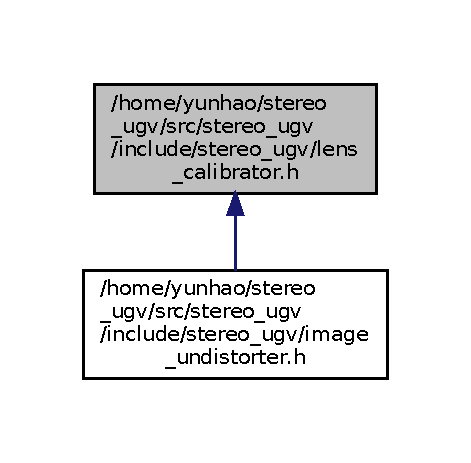
\includegraphics[width=226pt]{lens__calibrator_8h__dep__incl}
\end{center}
\end{figure}
\subsection*{Classes}
\begin{DoxyCompactItemize}
\item 
struct \hyperlink{structstereo__ugv_1_1LensCoefficients}{stereo\+\_\+ugv\+::\+Lens\+Coefficients}
\begin{DoxyCompactList}\small\item\em The structure of undistortion coefficients of a stereo camera. \end{DoxyCompactList}\item 
class \hyperlink{classstereo__ugv_1_1LensCalibrator}{stereo\+\_\+ugv\+::\+Lens\+Calibrator}
\begin{DoxyCompactList}\small\item\em The base class for calculating and saving undistortion coefficients of a stereo camera. \end{DoxyCompactList}\item 
class \hyperlink{classstereo__ugv_1_1ChessboardLensCalibrator}{stereo\+\_\+ugv\+::\+Chessboard\+Lens\+Calibrator}
\begin{DoxyCompactList}\small\item\em The class for calibrating a stereo camera using a chessboard pattern. \end{DoxyCompactList}\end{DoxyCompactItemize}
\subsection*{Namespaces}
\begin{DoxyCompactItemize}
\item 
 \hyperlink{namespacestereo__ugv}{stereo\+\_\+ugv}
\begin{DoxyCompactList}\small\item\em The namespace for public classes and functions of the Stereo U\+GV package. \end{DoxyCompactList}\end{DoxyCompactItemize}
\subsection*{Functions}
\begin{DoxyCompactItemize}
\item 
void \hyperlink{namespacestereo__ugv_aab7c44a98ba3f61baec2e4c1c9802bee}{stereo\+\_\+ugv\+::initialize} (Lens\+Calibrator $\ast$calibrator, const Context \&context)
\begin{DoxyCompactList}\small\item\em Initializes a \hyperlink{classstereo__ugv_1_1LensCalibrator}{Lens\+Calibrator}. \end{DoxyCompactList}\item 
void \hyperlink{namespacestereo__ugv_a8e8ff522fb8d2300fcdfc02ab0025e98}{stereo\+\_\+ugv\+::initialize} (Chessboard\+Lens\+Calibrator $\ast$calibrator, const Context \&context)
\begin{DoxyCompactList}\small\item\em Initializes a \hyperlink{classstereo__ugv_1_1ChessboardLensCalibrator}{Chessboard\+Lens\+Calibrator}. \end{DoxyCompactList}\end{DoxyCompactItemize}


\subsection{Detailed Description}
Defines \hyperlink{classstereo__ugv_1_1LensCalibrator}{stereo\+\_\+ugv\+::\+Lens\+Calibrator} and its subclasses. 


%--- End generated contents ---

% Index
\backmatter
\newpage
\phantomsection
\clearemptydoublepage
\addcontentsline{toc}{chapter}{Index}
\printindex

\end{document}
